%=======================================================
\section{Bridging the Physical and Digital Space}
%=======================================================

\subsection{\acl{DT} Modeling}
\label{sec:dt_modeling}
% Describe: physical interface, digital interface, model

% For an effective approach oriented towards interoperability and integration challenges of \ac{CPS} through the means of \acp{DT}, providing a clear modeling and general behavior is decisive.
Several approaches have been proposed to model \acp{DT} in different contexts~\cite{tao2022modeling}; hence, providing a comprehensive review is out of the scope of this work.
%
Since our proposal is grounded on the abstract \ac{DT} model originally presented in \cite{web-of-dt-ricci-2022}, in this section, we describe its main features.
%
We further recall other proposals from the scientific~\cite{dt-driven-prognostics-tao-2018,qi2021enablingtechdt,requirements-patterns-dt-industry-bellavista-2023} and standardization communities~\cite{etsi-dt-comm-requirements-2024} 
aligning it with the work presented in \cite{web-of-dt-ricci-2022} to provide a background on \ac{DT} modeling.


\subsection{Digital Twin Abstract Architecture}

Among the most recognized models for \acp{DT}, Tao's 5D model~\cite{qi2021enablingtechdt},
%(Figure~\ref{fig:tao_mapping_dt_modelling}, left),
defines five fundamental dimensions a \ac{DT} must have: the physical entity (PE), virtual entity (VE), connection (C), data (DD) and services (SS) dimensions.
The model can be mapped into an abstract software architecture (which is a generalization of the one proposed in \cite{web-of-dt-ricci-2022})
structured with three main components, as depicted in Figure \ref{fig:dt_application_example}: i) \emph{\ac{PI}}: takes care of the connection (C) and synchronization with the physical entity (PE); ii) \emph{Model (M)}: data gathered by the PI is passed to the \ac{DT} models, which elaborate it, implementing the virtual entity (VE) absolving to the digitalization purpose of the \ac{DT} and storing relevant data (DD); and iii) \emph{\ac{DI}}: exposes the \ac{DT} model computation results as well as endpoints for action and query requests to external entities as services (SS), creating a connection (C) between the \ac{DT} and digital applications.

% \begin{itemize}
%     \item \emph{\ac{PI}}: takes care of the connection (C) and synchronization with the physical entity (PE);
%     \item \emph{Model (M)}: data gathered by the PI is passed to the \ac{DT} models, which elaborate it, implementing the virtual entity (VE) absolving to the digitalization purpose of the \ac{DT} and storing relevant data (DD).
%     \item \emph{\ac{DI}}: exposes the \ac{DT} model computation results as well as endpoints for action and query requests to external entities as services (SS), creating a connection (C) between the \ac{DT} and digital applications.
% \end{itemize}

%%%
% \begin{figure}[ht]
%     \setlength{\belowcaptionskip}{-13pt}
%     \centering
%     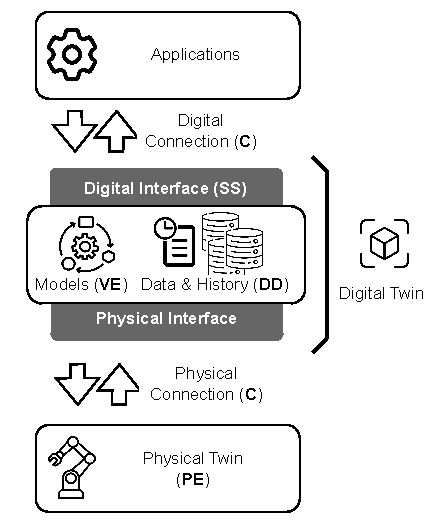
\includegraphics[width=0.6\columnwidth]{images/dt-model.pdf}
%     \caption{A Digital Twin abstract architecture inspired by Tao's 5D model.}
%     \label{fig:dtmodel}
% \end{figure}
%%%

% In the abstract architecture depicted, \emph{physical entity} is \emph{connected} to its \emph{digital representation} by the interfaces involved, with the PI ensuring proper communication with the \ac{DT} Model, and the DI enabling communication with the upper level \emph{digital services} interested in the context of the \ac{DT}.

Internally, a process identified as \emph{twinning} or \emph{shadowing}~\cite{saracco2019dt,web-of-dt-ricci-2022} handles the transformation of data received from the PI, feeding the models that characterize the \ac{DT}. The result of the shadowing process is to compute the state of the \ac{DT}, which can be represented as a set of: i) \textbf{Properties}: labeled data that change with the evolution of the physical counterpart state; ii) \textbf{Events}: non-persistent signals captured by the information gathered from the associated physical asset; iii) \textbf{Relationships}: capturing the existing and dynamic connections among physical assets within the system, mirroring them between the corresponding \acp{DT}; and iv) \textbf{Actions}: the set of possible operations that the \ac{DT} allows to invoke on behalf of the physical counterpart, to either send feedback to the physical entity or exploit a service exposed by the \ac{DT}~\cite{web-of-dt-ricci-2022}.
% \begin{itemize}
%     \item \textbf{Properties}: labeled data that change with the evolution of the physical counterpart state;
%     \item \textbf{Events}: non-persistent signals captured by the information gathered from the associated physical asset;
%     \item \textbf{Relationships}: capturing the existing and dynamic connections among physical assets within the system, mirroring them between the corresponding \acp{DT}; and
%     \item \textbf{Actions}: the set of possible operations that the \ac{DT} allows to invoke on behalf of the physical counterpart, to either send feedback to the physical entity or exploit a service exposed by the \ac{DT}~\cite{web-of-dt-ricci-2022}.
% \end{itemize}
%
State updates can then be communicated to applications through the \ac{DI}, fulfilling the objective of the \ac{DT} in providing an up-to-date representation of the \ac{PT}.
%
The digital invocation of actions on the \ac{DT} is also converted to the appropriate physical actuation through the shadowing process, achieving bi-directional synchronization~\cite{web-of-dt-ricci-2022}.
% \emph{properties}, \emph{events}, \emph{relationships}, and \emph{actions}.
% \begin{itemize}
%     \item \textbf{Properties} collect and expose all the labeled data that change with the evolution of the physical counterpart state;
%     \item \textbf{Events} model non-persistent signals captured by the information gathered from the associated physical asset;
%     \item \textbf{Relationships} model and capture the existing and dynamic connections among physical assets within the system, mirroring them between the corresponding \acp{DT};
%     \item \textbf{Actions} expose the set of possible operations that the \ac{DT} exposes on behalf of the physical counterpart, to either send feedback to the physical entity or exploit a service exposed by the \ac{DT}.
% \end{itemize}

% %%%
% \begin{figure*}[t]
%     \centering
%     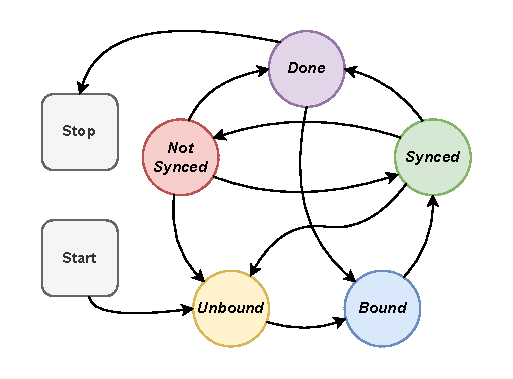
\includegraphics[width=0.70\textwidth]{images/wldt-lifecycle.pdf}
%     \caption{A visual representation of the lifecycle of a \acl{DT}.}
%     \label{fig:life_cycle}
% \end{figure*}
% %%%


\subsection{Engineering \acl{DT} Interoperability}
\label{sec:engineering-interoperability}

Figure \ref{fig:dt_application_example} represents a \ac{DT} implemented following the abstract architecture presented in Section \ref{sec:dt_modeling} in an exemplary deployment setting.
It highlights the role of the \ac{DT} as a bridge between \emph{physical} devices and \emph{digital} applications.
% By abstracting the complexity of connecting with the \ac{PT}, the \ac{DT} provides a digital replica tailored to application-specific requirements.

At an appropriate abstraction level, a \ac{PT} may be digitalized by obtaining and sending data through possibly \emph{several} different \texttt{Communication Channels}, which 
encompass network protocols, data formats, and physical connections.
The \ac{PI} manages interactions with the \ac{PT}, integrating such channels.
%
Similarly, on the digital side, the \ac{DT} supplies data and insights to applications via the \ac{DI}, adapting to different protocols and representations.

% Engineering the \ac{PI} and \ac{DI} requires addressing the challenge of effectively integrating such heterogeneous communication channels.
%
We argue that to ensure flexibility and adaptability, it is essential that the core of the \ac{DT}, including its models and implemented behaviors, remains decoupled from the heterogeneous physical and digital communication channels.% involved in interacting with \acp{PT} and applications.
%
The \ac{DT}'s shadowing process should focus solely on understanding the available physical data, receiving and transmitting telemetry information, and executing action requests, with no concern for the underlying implementation details.
%
This separation of concerns should be supported by the \ac{DT} architecture and achieved through a modular design of the \ac{DT} components, which has been proven effective~\cite{requirements-patterns-dt-industry-bellavista-2023,bellavista2024fgcs} as it strengthens extensibility, interoperability and maintainability with respect to monolithic approaches.

In the remainder of this section, we present our proposal for the design the \ac{DT}'s \ac{PI} and \ac{DI}, refining and extending the conceptual model originally proposed in \cite{web-of-dt-ricci-2022} with a concrete implementation based on the concept of modular \emph{adapters}.

\subsection{Physical Interoperability}
\label{sec:physical_interoperability}

%%%
\begin{figure}[t]
    \centering
    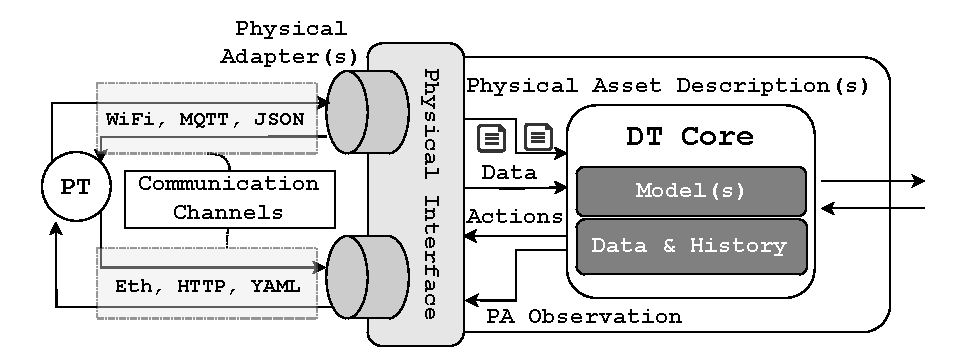
\includegraphics[width=\columnwidth]{figures/dt-interoperability/dt_interoperability_physical.pdf}
    \caption{PI design with modular physical adapters each producing the corresponding \acl{PAD} that is processed by the \ac{DT} Model.}
    \label{fig:physical_interoperability}
\end{figure}


% %\afterpage{%
% \begin{figure}[h!]
%   \setlength{\belowcaptionskip}{-5pt}
%   \centering
%   \begin{subfigure}{0.5\linewidth}
%       \centering
%       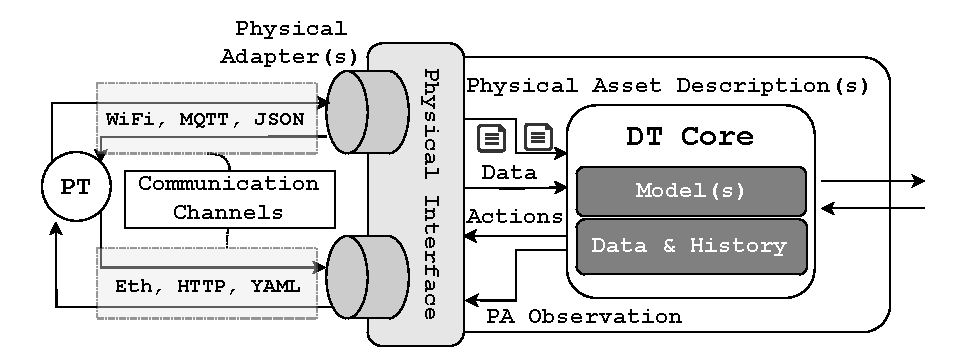
\includegraphics[width=\linewidth]{figures/dt-interoperability/dt_interoperability_physical.pdf}
%       \caption{Physical Interface}
%       \label{fig:physical_interoperability}
%   \end{subfigure}
%   \begin{subfigure}{0.5\linewidth}
%       \centering
%       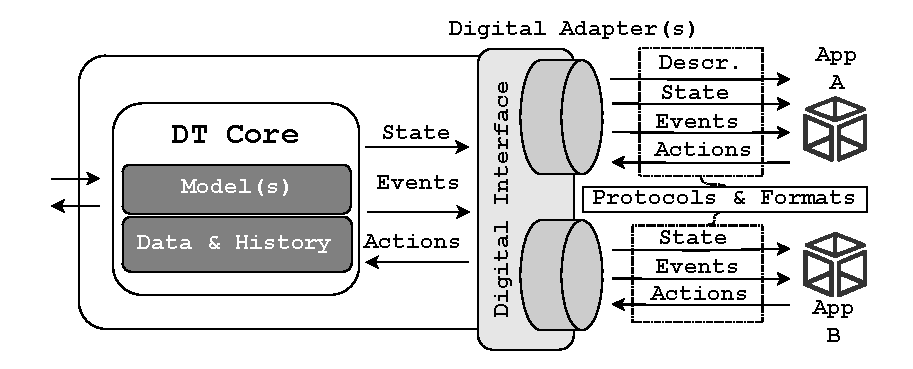
\includegraphics[width=\linewidth]{figures/dt-interoperability/dt_interoperability_digital.pdf}
%       \caption{Digital Interface}
%       \label{fig:digital_interoperability}
%   \end{subfigure}
  
%   \caption{DT interfaces and their responsibilities to enable and support cyber-physical interoperability.}
%   \label{fig:benchmark_webapp}
% \end{figure}
% %}

One of the main challenges in facilitating effective communication through the \ac{PI} is the wide variety of communication protocols and data formats used by \acp{PT}.
%
While it can be the case that one \ac{PT} is directly sending all the data concerning its digitalization through only one channel,
it is far more common to build a \ac{DT} aggregating different sources of information~\cite{qi2018dt-and-bigdata}.
%
\ac{IoT} protocols often differ considerably based on the manufacturer, device type, or application domain, making it difficult for the \ac{DT} software to integrate diverse assets.

% Regardless of the underlying complexity,
% from an engineering perspective,
% it is essential to decouple the \ac{DT} model from the communication requirements of the \ac{PT}.
%
We argue that the modularity of the \ac{PI}, which encapsulates these responsibilities, is a crucial factor in the design and implementation of interoperable \acp{DT}.
%
Hence, we propose the \ac{PI} to be designed as composed of multiple \emph{\acp{PhA}}: specialized modules capable of interacting with the \ac{PT} using diverse protocols and data formats.
%
As shown in Figure \ref{fig:physical_interoperability}, each \ac{PhA} is responsible for mediating the bi-directional interaction through a single communication channel, simplifying the design and reusability of the component, and making it configurable to adapt to different application contexts.
%
The responsibility of the \ac{PI} becomes then to manage the different \acp{PhA} and make sure the \ac{DT} model can accurately interpret, process, and leverage the data generated by the physical world to create the digital replica and implement its behaviors.
%
Note that although we borrow the terminology of \ac{PhA} from \cite{web-of-dt-ricci-2022}, where it is originally introduced, our proposal differs significantly.
The \emph{Physical Asset Adapter} proposed in \cite{web-of-dt-ricci-2022} is infact a conceptual monolithic component, whereas in our concrete proposal, we consider a \ac{PhA} as a single-responsibility module of a potentially more complex \ac{PI}.

\subsubsection{Generating \aclp{PAD}}
To facilitate the process of managing different \acp{PhA}, we introduce the idea of generating a \emph{\ac{PAD}}: a representation of the capabilities made available by a communication channel in terms of \emph{properties}, \emph{actions}, \emph{events} and \emph{relationships} that characterize the associated \ac{PT}.
%
Each \ac{PhA}, since it encapsulates the characteristics of a channel, can generate the corresponding \ac{PAD}, effectively decoupling the asset's functionality from the specific communication protocols used.
%
The implementation of the \ac{PAD} generation can be challenging due to the varying capabilities of different communication protocols.
For instance, protocols like CoAP\cite{RFC7252} often come with built-in description and discovery functionalities, which can simplify the process of creating a \ac{PAD} by providing standardized representations of the physical asset's capabilities and behaviors.
On the other hand, protocols like MQTT may require developers to add additional information manually to define how information is structured and exchanged, as they do not natively include asset metadata \cite{mqtt}.
In the case of custom or proprietary protocols, the challenge becomes even more pronounced, as these protocols are tailored to specific systems and may lack any standardization or descriptive capabilities.

In all the aforementioned scenarios, the mechanism of \ac{PAD} generation offers a way to encode knowledge about the \ac{PT} bridging the gap by interpreting and extracting relevant information from the protocol used in the associated communication channels.
%
Confining this complexity within the \ac{PI} allows the \ac{DT} model to be agnostic with regard to the complexity of the underlying physical world.

The \ac{PAD} allows the \ac{PI} to discover, extract, and manage asset information and present it to the model that can choose which ones are relevant for the implementation of the \ac{DT} behavior.
%
For example, to create the \ac{DT} of a temperature sensors streaming binary data on MQTT, the \ac{PI} could be composed of a generic MQTT adapter, configured to correctly parse the payload as a decimal number, and generate a \ac{PAD} which advertise the available temperature property to the \ac{DT} model as a Celsius value. 

\subsubsection{\aclp{PAD} in the \ac{DT} Lifecycle}

The modular design of the \ac{PI} has an impact on the \ac{DT} lifecycle presented in Figure \ref{fig:lifecycle}.
%
Specifically, it tackles the open challenge of transitioning from the \texttt{Unbound} to the \texttt{Bound} state.
%
When a \ac{PhA} successfully connects to the \ac{PT}'s channel and starts receiving data from it, it can send the generated \ac{PAD} to the \ac{DT} model.
The generation of the \ac{PAD} can be used as a synchronization step to signify that the \ac{PhA} is successfully connected to the \ac{PT}.
%
The \ac{DT} model is then responsible for collecting the different \acp{PAD}, assessing whether all the relevant information to start computing the \ac{DT} state is available and, hence, moving on to the \texttt{Bound} phase.
%
This mechanism enables managing the \ac{DT} behavior consistently, even with the additional complexity of the modular \ac{PI} design.


\subsection{Digital Interoperability}
\label{sec:digital_interoperability}

%%
\begin{figure}[t]
    \centering
    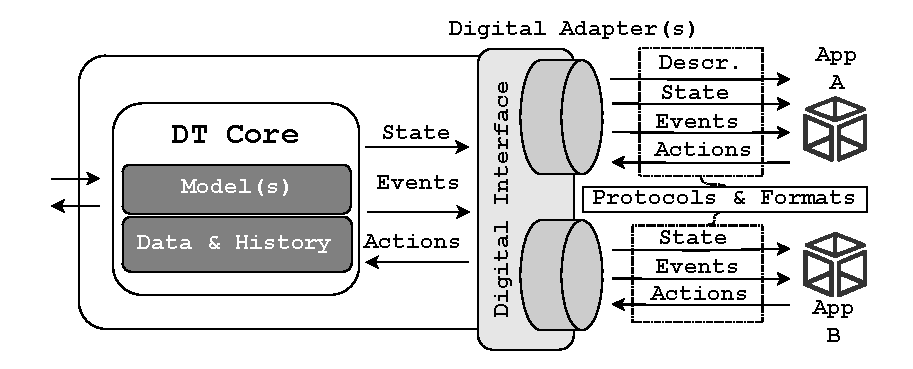
\includegraphics[width=\columnwidth]{figures/dt-interoperability/dt_interoperability_digital.pdf}
    \caption{Digital Interface design with adapters and DT description, state and sync.}
    \label{fig:digital_interoperability}
\end{figure}
%%

As \acp{DT} are meant to bridge between the physical and digital spaces,
interoperability is not only a matter of interfacing with heterogeneous devices, but also other digital applications.
Indeed, despite their initial conception as vertical silos, the concept of Digital Twins Ecosystems~\cite{web-of-dt-ricci-2022,kendall2021ndt} is emerging to support the the digitalization of complex scenarios through a combination of several \acp{DT}.
%
In this context, \acp{DT} can be used \emph{as-a-service}~\cite{liu2022state} by other applications implementing the business logic by spanning across different software entities.

To foster interoperability in ecosystems, \acp{DT} must then expose either a standardized general purpose \acf{DI} that can serve different applications or
-- following the same design principles adopted to address physical interoperability --
have a modular interface that can satisfy the different needs of different applications
as shown in Figure \ref{fig:digital_interoperability}.

As for \ac{PhA} we borrow the terminology from \cite{web-of-dt-ricci-2022} and consider to have a \ac{DI} composed of modular \ac{DiA}.
We thus refine the original abstract concept of \ac{DiA} to represent a modular component of a more complex \ac{DI}.
Using the concept of \ac{DiA}, the \ac{DI} can expose the \ac{DT} state and services supporting multiple data formats and interaction patterns.
This can be beneficial for integrating it with applications and, especially, legacy systems.
The existence of legacy applications usually implies having little control over the integration requirements, making having more flexible \acp{DT} beneficial to better integrate with the application requirements.
% %
% One of the benefits of adopting a \ac{DT}-based design is their bridging role, shielding applications from the complexity of physical deployments.
% %
% As described in the previous section, \acp{DT} can decouple from the communication channels.
% %
% Hence, applications can leverage the \ac{DT} unified \ac{DI} instead of hardcoding against the possibly several communication channels of the \ac{PT}.
%
Using several \ac{DiA}, a \ac{DT} could, for instance, support both request-response and publish-subscribe mechanisms to access its current and previous states, support different query languages to access the same data store, expose its current state using different representation formats, etc.
%
This would make the development of the application simpler because adding an application-specific \ac{DiA} won't require intervention in the underlying physical system. 
%
Additionally, the developed application would be more robust and stable since it would depend only on the \ac{DT}, and changes to the physical configuration of the \ac{PT} (e.g., software updates, sensor replacement, network reconfigurations) would have no impact on the application software.
%
Even if the \ac{PT} were to change, (e.g., a software update on a robot changes the telemetry format) the \ac{DI} of the \ac{DT} could stay the same, as the changes would occur within the boundaries of the \ac{PI} and \ac{DT} model.
%
Through this mechanism, \acp{DT} effectively achieve their bridging role, shielding applications from the complexity of physical deployments.

\subsubsection{Describing \aclp{DI}}

A further level of interoperability is possible when allowing \acp{DT} to describe their \ac{DI}, advertising capabilities and available communication channels that applications can exploit.
%
% This is especially relevant in contexts where applications are not bound to a specific interface but can instead process machine-readable descriptions of \acp{DT} and choose to interact with specific assets.
%
A \ac{DT} could then use a \emph{\ac{DTD}}, which, similarly to the \ac{PAD}, can represent the features of the \ac{DT} to its observers.
%
The idea of exposing \acp{DTD} is somewhat present in the major platforms supporting the creation of \ac{DT} ecosystems, such as 
Microsoft's Azure Digital Twins\footnote{\url{https://azure.microsoft.com/en-us/products/digital-twins}} and Eclipse Ditto\footnote{\url{https://eclipse.dev/ditto/}} and is advocated by research works on interoperability in \ac{DT} ecosystems~\cite{etsi-dt-comm-requirements-2024,giulianelli2024models}.

The way such descriptions are implemented may differ significantly, but essentially, they should at least allow representing the \ac{DT}  features and APIs to access them.
%
Notably, differently from the \ac{PAD}, the \ac{DTD} is targeted to external consumers, hence, it should preferably adhere to standard formats and representations to be useful in practice in achieving interoperability.
%
To this end, using Linked Data principles\footnote{Original definition of the Linked Data principles: \url{https://www.w3.org/DesignIssues/LinkedData.html}} could be a possible solution to implement standard machine-readable \acp{DTD}~\cite{burattini2024models}.

\begin{figure*}[t]
    \setlength{\belowcaptionskip}{-13pt}
    \centering
    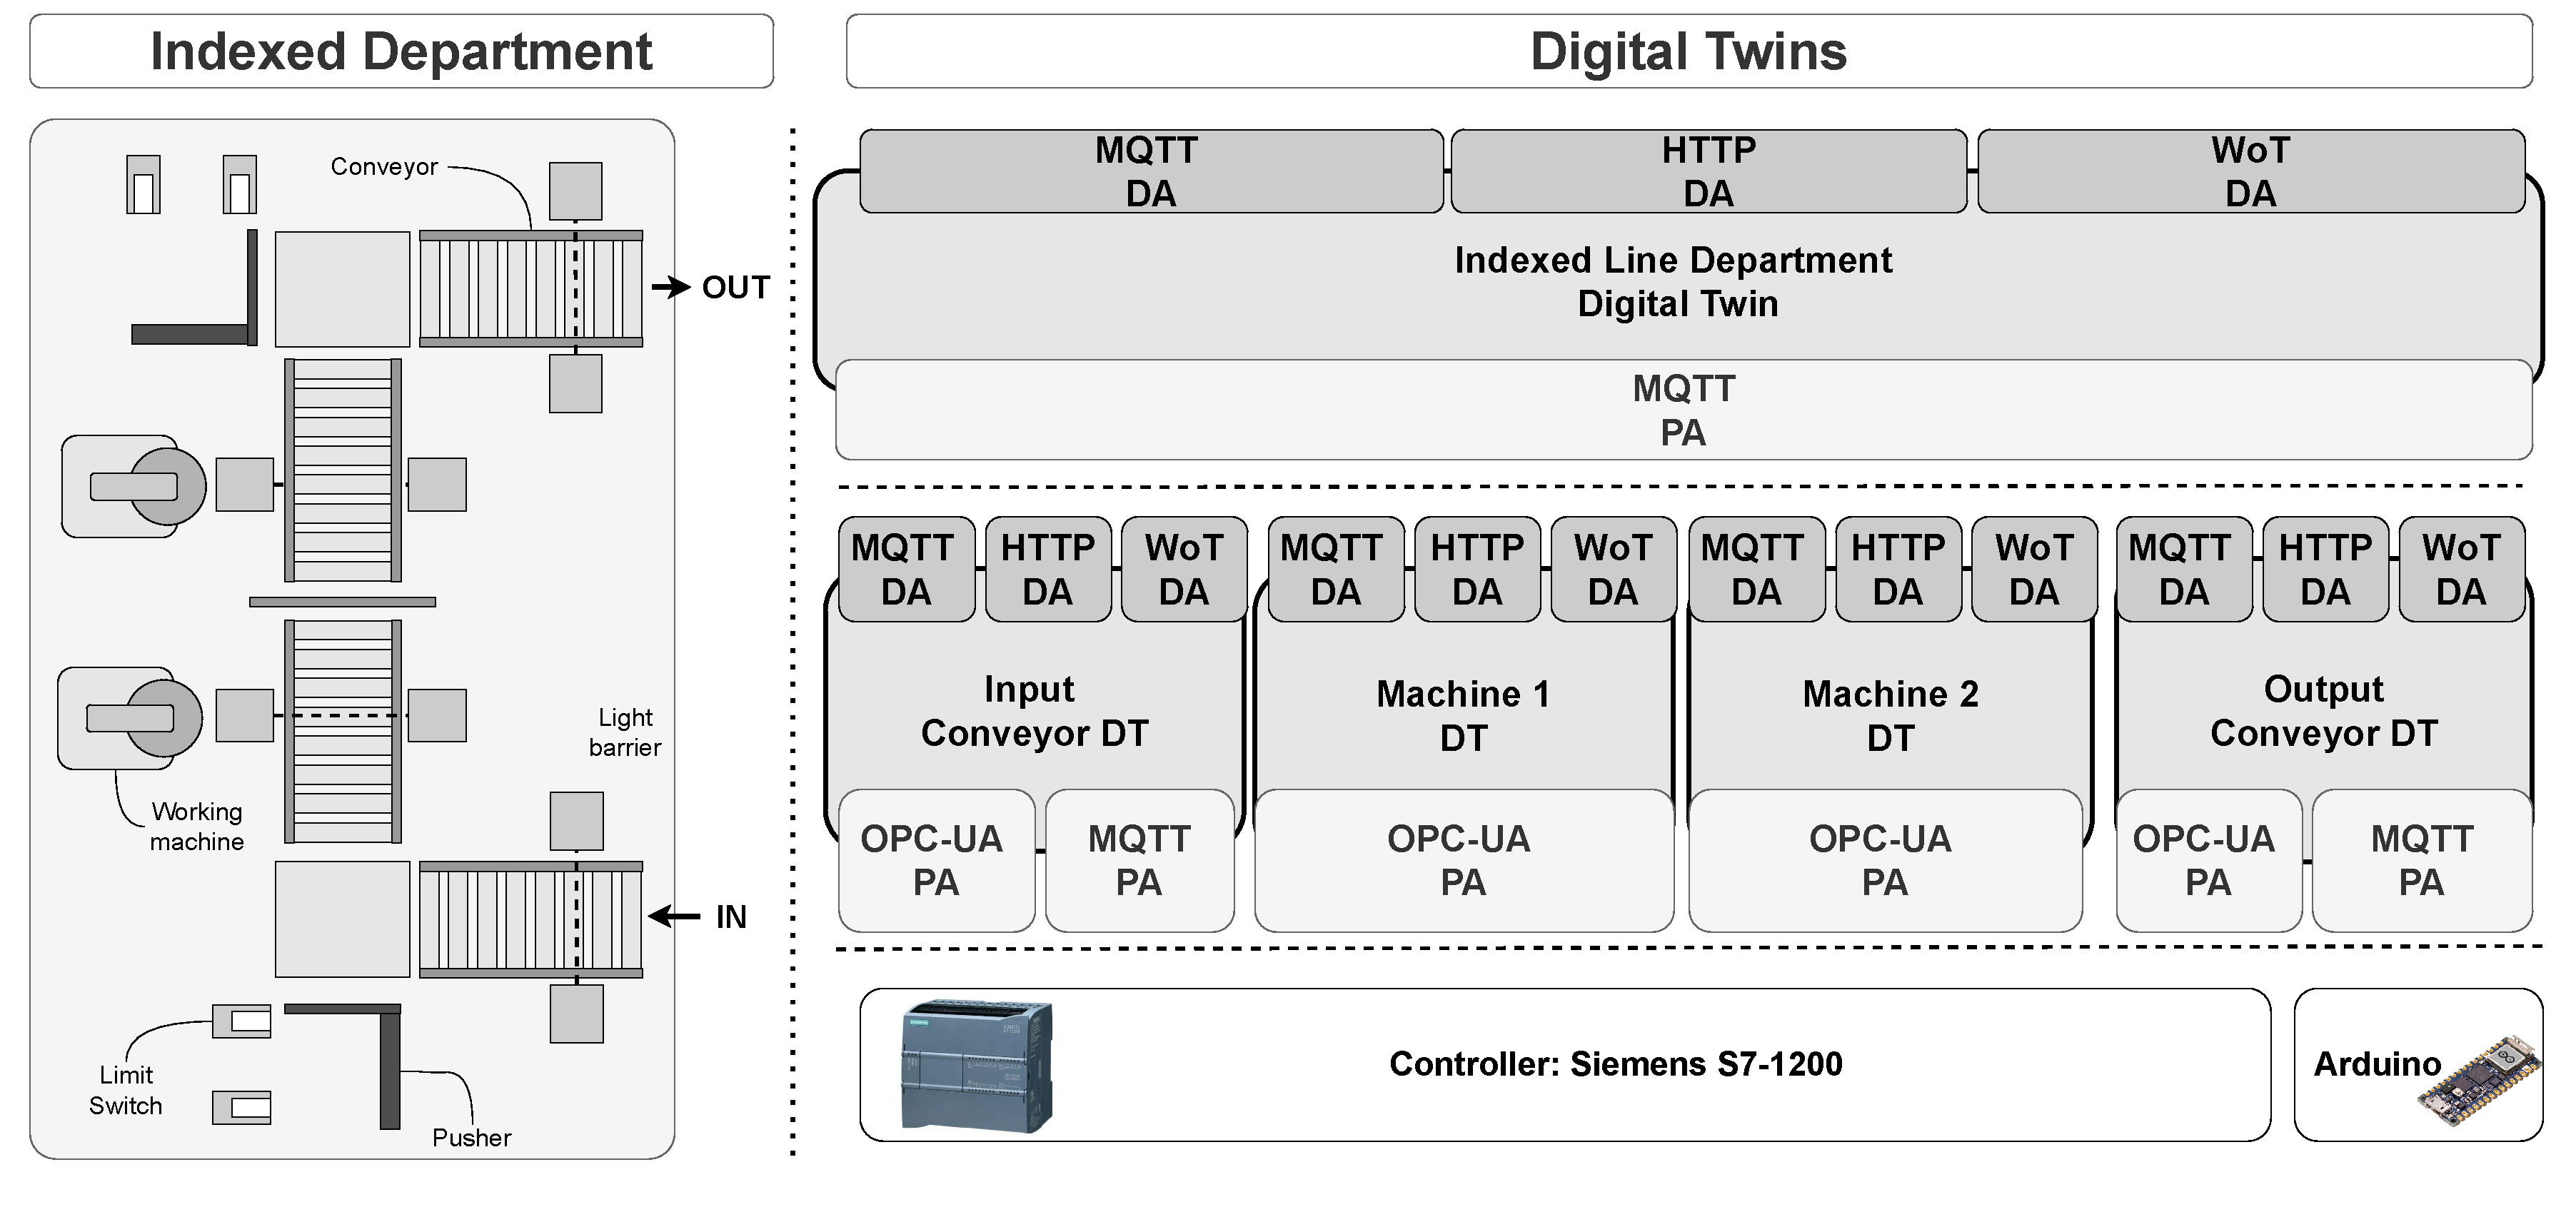
\includegraphics[width=0.93\linewidth]{figures/dt-interoperability/mf_dt_structure.pdf}
    \caption{The \acl{DT} ecosystem architecture of the microfactory industrial system.}
    \label{fig:mf_dt_ecosystem}
\end{figure*}

\subsection{\acl{WoT}: enabling \ac{DT} Interoperability}
\label{sec:wot-dt-interop}

Tackling interoperability in the \ac{IoT} context is not a novel issue.
Before the emergence of \acp{DT} several solutions have attempted to solve it through the definition of standards~\cite{lee2021iot-interoperability-standards}.

In this section, we analyze the set of standards produced for the \ac{WoT}~\cite{wotarch} as they share the goal of our proposal of adopting uniform API and data format descriptions to hide low-level complexities and promote interoperability.

In the context of the \ac{WoT}, \textit{Things} represent abstractions over physical or virtual entities that participate in the \ac{WoT}~\cite{wotarch}.
\ac{WoT} Things are described in terms of metadata and interfaces by the \ac{WoT} \ac{TD}~\cite{wotthing}.
%serves as a standardized blueprint for a physical object, specifying its \emph{interaction affordances}.
A \ac{TD} provides a machine-readable blueprint for describing metadata and \textit{interaction affordances} of a physical object \cite{wotthing}.

Despite their similarities, \acp{PAD} and \acp{TD} serve distinct purposes. 
A \ac{TD} provides a structured description of a physical twin's available interactions to external consumers, detailing protocols and interaction possibilities.
%
In contrast, a \ac{PAD} is designed for internal use within the \ac{DT} modules, decoupling the twin's core from the complexities of communication channels.
Its primary role is to facilitate the discovery of available resources and capabilities on the \ac{PT} after establishing a connection with the physical counterpart, providing a structured description of its functionalities and data.
This description is directly interpretable by the \ac{DT} model while remaining independent of the physical characteristics, allowing, for instance, the reuse of the same model for similar \acp{PT} employing different communication approaches.

In those context in which \ac{WoT} standards are applicable, the devices' \acp{TD} can be automatically mapped to \acp{PAD}, streamlining the \ac{DT} creation process.
% This mapping enhances the interoperability between digital and physical systems, as the \ac{PAD} provides a structured representation of the asset’s functionalities, ensuring seamless integration into the \ac{DT} framework.
%
% Leveraging \ac{WoT} \acp{TD} can significantly reduce the effort required to generate \acp{PAD}, particularly in environments where numerous physical twins already have associated \acp{TD}.
This convergence between \ac{WoT} and \ac{DT} architectures has the potential to accelerate the development and deployment of \ac{DT} solutions by promoting standardization and reusability.
%
Nevertheless, the more general concept of \ac{PAD} can be tailored also to those scenarios in which \ac{WoT} is not applicable. In those cases the responsibility falls back to development (or configuration) of a \ac{PhA} for a specific device to encode the necessary knowledge for the generation of the \ac{PAD}.

% In contrast, a \ac{PAD} plays a more dynamic role within a \ac{DT}, not only facilitating data exchange but also enabling higher-level functionalities, such as triggering actions and implementing advanced behaviors that extend beyond direct physical mappings.
% The \ac{DT} core leverages the \ac{PAD} to interpret and augment physical data, supporting richer and more complex digital representations.

\ac{WoT} \acp{TD} can also be used as \acp{DTD}.
The \ac{WoT} architecture actually lists \acp{DT} as one of the possible deployment patterns, with a \ac{DT} mediating the interaction with a \ac{PT} behind a \ac{WoT} interface~\footnote{\url{https://www.w3.org/TR/2023/REC-wot-architecture11-20231205/\#digital-twins}}.
%
This is especially useful when devices are not \ac{WoT} compatible or can not be made so due to other constraints, essentially retrofitting the capabilities of the devices with a \ac{WoT} compatible interface.
%
Adhering to REST constraints~\cite{fielding2002rest} -- the architectural style of the Web -- and specifically to the HATEOAS and self-descriptive principles, a \ac{TD}-based \ac{DTD} facilitates the discovery of the \ac{DT} model and services.
%
Its machine-readable nature ensures interoperability for applications and consumers.
%
In particular, a \ac{TD}-based \ac{DTD} facilitates the inclusion of \acp{DT} in \ac{WoT} mashups, promoting \acp{DT} as valid \ac{WoT} Things usable by \ac{WoT} Consumers.

Despite its flexibility,
%and broad applicability, 
using of \ac{TD} for \acp{DT} presents several limitations in capturing the specific characteristics of \acp{DT} that distinguish them from \emph{Things}~\cite{burattini2024models}.
A path to address these limitations could be extending \acp{TD} or supporting additional descriptions specifically for \acp{DT} in \ac{DT} ecosystem \cite{giulianelli2024models}.



%=======================================================
\section{Managing the Digital Twin Lifecycle}
%=======================================================


Recently, there has been an increasing recognition of the importance of the lifecycle of \acp{DT}, particularly in distinguishing the properties that define the relationship between the \ac{DT} and \ac{PT}. Key concepts such as \emph{reflection} and \emph{entanglement} are critical for accurately representing the \ac{PT}~\cite{dt-IoT-context-Minerva-2020, web_of_dt}. These properties underscore the necessity for a structured lifecycle for the \ac{DT}, ensuring that its state remains consistently aligned with the \ac{PT} throughout various stages. As highlighted in a recent survey~\cite{ferko2022architecting, 9640612, HRIBERNIK2021103508}, while the body of literature on \ac{DT} software architectures is growing, most papers are domain-specific and focus on reference models~\cite{1999daglib}. However, these models often lack concrete guidance on how to implement the internal components of a \ac{DT}. Many of the existing models envision multiple parallel components or models working together, but fail to address how they communicate and interact to maintain consistency in the \ac{DT} state. This gap leads to potential inconsistencies between the \ac{DT} and \ac{PT}, as the interaction between models and the management of state changes is not adequately captured~\cite{alam2017access,Malakuti2019fourlayer,Lpez2021}.

In \cite{Redelinghuys2019}, a six-layer architecture for \acp{DT} is proposed, where the first two layers are dedicated to the \ac{PT} (sensors and controllers), and the third to the fifth layers manage data storage, communication, and cloud integration. However, the architecture lacks a clear process for how these layers communicate with each other or how changes in the \ac{DT} state are captured and updated across the layers. Similarly, in the Generic \ac{DT} Architecture (GDTA)~\cite{app10248903}, a layered approach is used, where the \ac{DT} state is computed at the \emph{information layer} through data processing pipelines. However, this architecture does not incorporate an explicit mechanism for the integration of the different components of the \ac{DT}, leaving gaps in how the evolving state of the \ac{DT} is managed. Other models explicitly reference multiple components that contribute to the definition of the \ac{DT} state. For example, in \cite{alam2017access} and similarly in \cite{Malakuti2019fourlayer}, the authors propose multi-layer \ac{DT} architecture for cyber-physical systems (CPS), where \ac{DT} state changes are driven by multiple functional units. However, in these models, the outputs of each unit are not mediated by a shadowing process, which would ensure consistency and synchronization of the \ac{DT} state and lifecycle management. Our approach addresses these issues by proposing a more structured lifecycle for \acp{DT}, where the communication and interaction between the different components are clearly defined. By introducing a shadowing process that orchestrates the different models, we ensure that the \ac{DT} state remains consistent and accurately reflects the evolving state of the \ac{PT}.


\subsection{Digital Twin Lifecycle}

A \ac{DT} is a ``living'' software entity:
The concept of \ac{DT} lifecycle, as introduced in~\cite{web-of-dt-ricci-2022}, covers the various phases a \ac{DT} undergoes from creation to deactivation, focusing on its synchronization with the \ac{PT}.
The phases are illustrated in Figure \ref{fig:lifecycle}.
% The lifecycle includes the phases:
% \texttt{Started},
% \texttt{Unbound},
% \texttt{Bound},
% \texttt{Synchronized},
% \texttt{Out of Sync},
% \texttt{Done},
% and \texttt{Stopped},
% detailing the \ac{DT}'s interaction with the \ac{PT} and its software behavior.
The \ac{DT} transitions from the \texttt{Unbound} phase, where internal modules are prepared, to the \texttt{Bound} phase once it successfully binds with the \ac{PT}.
In the \texttt{Synchronized} phase, the \ac{DT} maintains an up-to-date digital replica of the \ac{PT}.
If synchronization fails, the \ac{DT} enters the \texttt{Out of Sync} phase until issues are resolved.
When the \ac{DT} is no longer required, it transitions to the \texttt{Done} phase, then to \texttt{Stopped}.
Errors or reboots may lead back to the \texttt{Unbound} phase.

The transition from the Unbound to Bound phase in the \ac{DT} lifecycle remains an open research area:
a key challenge is identifying whether all the capabilities of the \ac{PT} relevant to support the \ac{DT}'s behavior are available so that the shadowing process can start.
We further elaborate on how to tackle this challenge with our contribution in Section~\ref{sec:physical_interoperability}.

%%%
\begin{figure}[ht]
    \setlength{\belowcaptionskip}{-13pt}
    \centering
    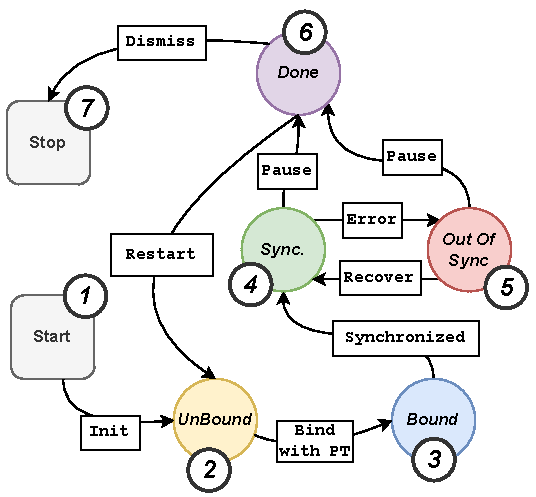
\includegraphics[width=0.8\linewidth]{figures/dt-interoperability/dt-lifecycle.pdf}
    \caption{\acl{DT} lifecycle phases and transactions.}
    \label{fig:lifecycle}
\end{figure}

\begin{figure*}[t]
    \setlength{\belowcaptionskip}{-13pt}
    \centering
    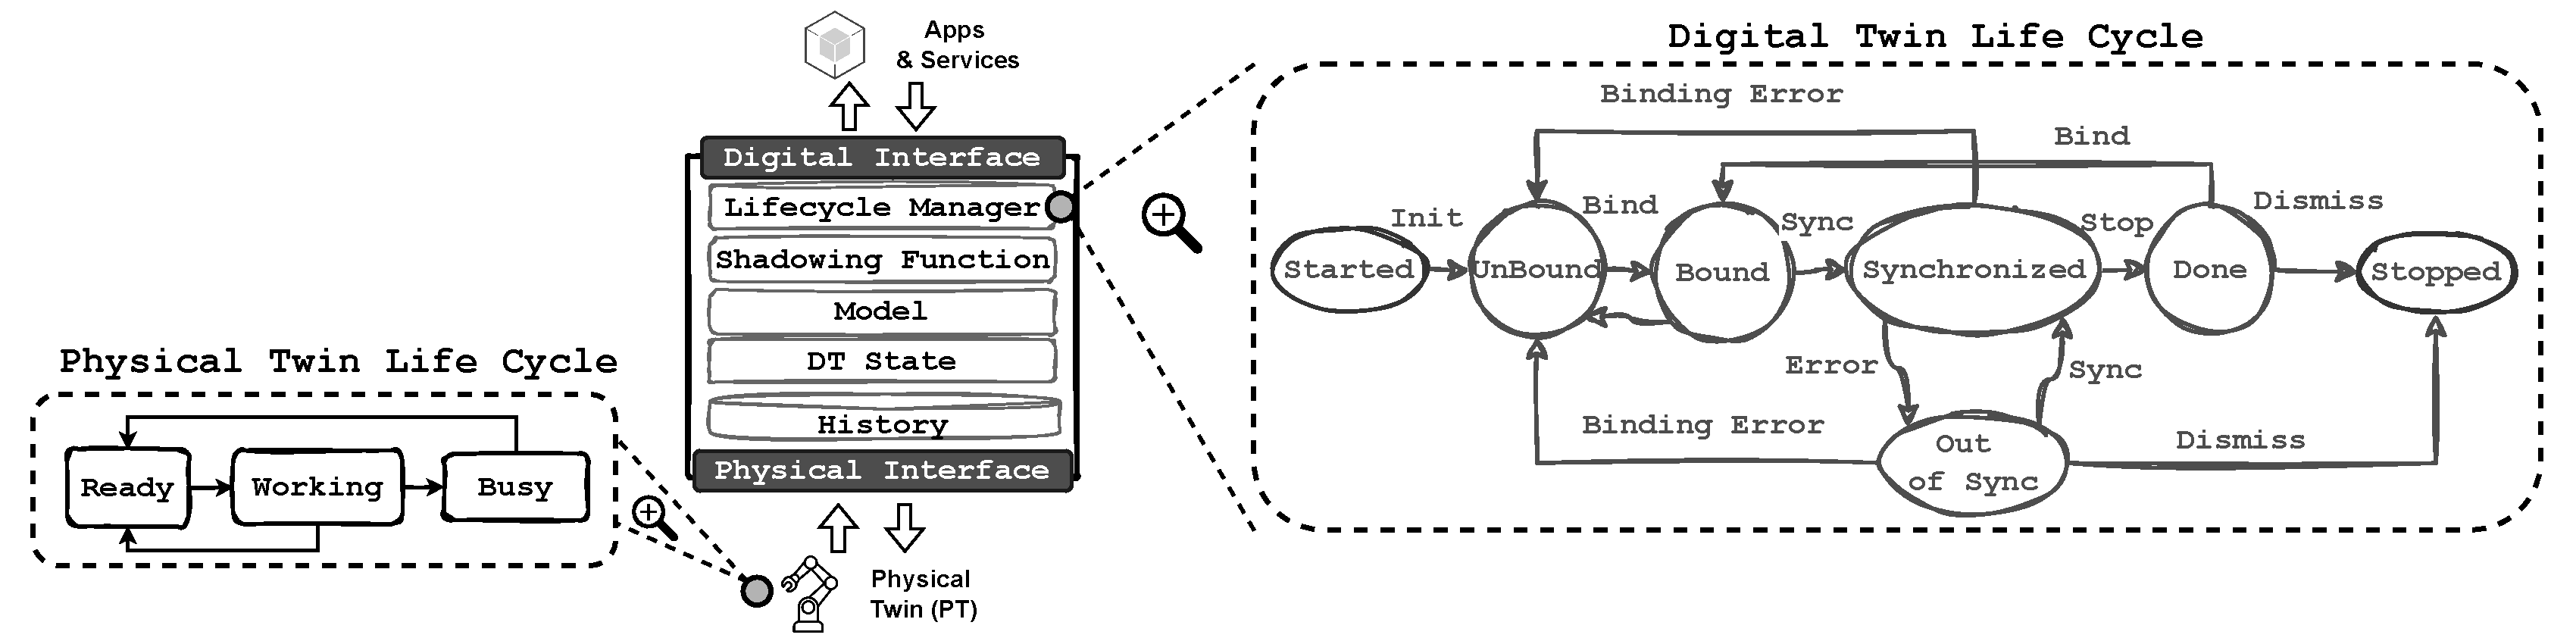
\includegraphics[width=\textwidth]{figures/dt-lifecycle/dt_model_lifecycle_dt_pt.pdf}
    \caption{A schematic representation of a DT, emphasizing its lifecycle alongside that of its physical counterpart.}
    \label{fig:dt_model_pt_dt_lifecycles}
\end{figure*}


\begin{figure*}[t]
    \setlength{\belowcaptionskip}{-13pt}
    \centering
    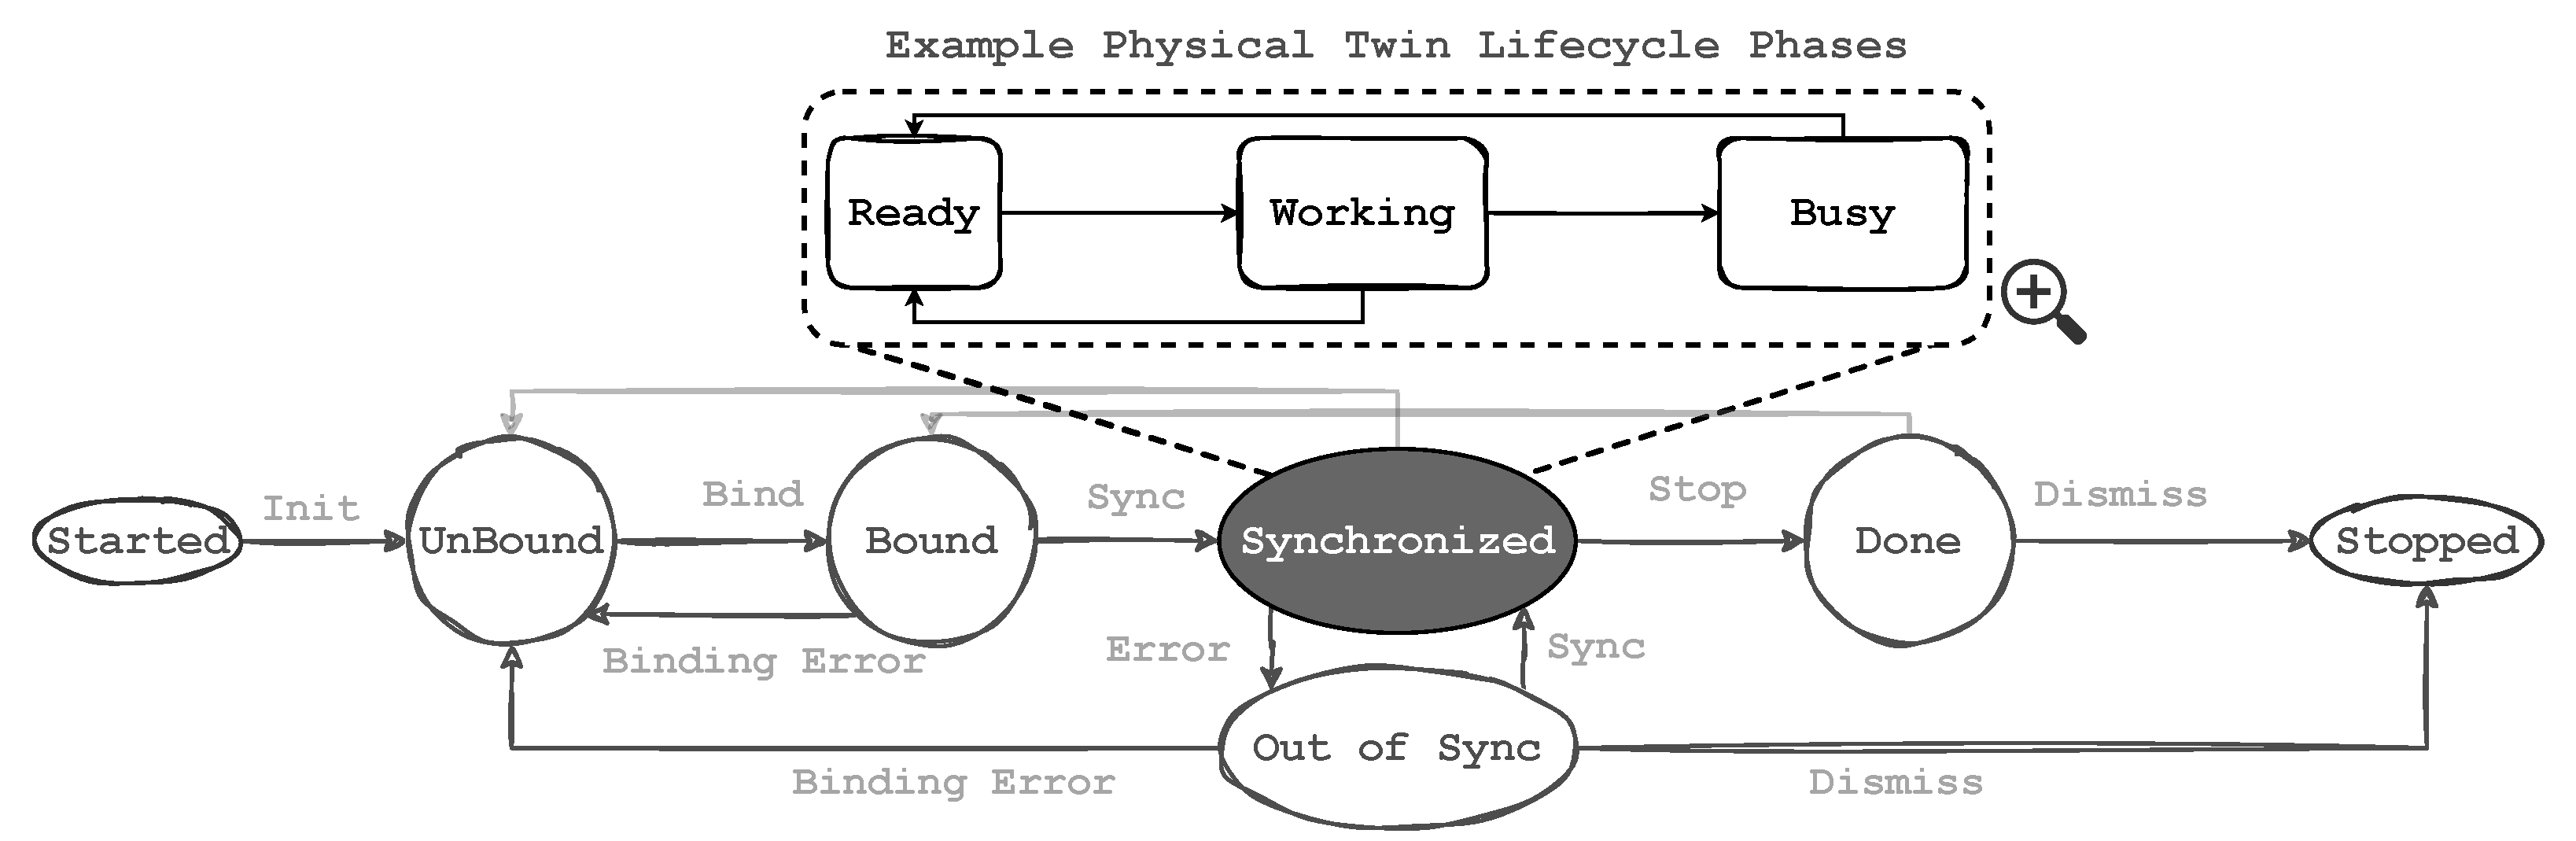
\includegraphics[width=\textwidth]{figures/dt-lifecycle/dt_lifecycle_pt_sync.pdf}
    \caption{Schematic representation of the DT lifecycle with a structured example of the Synchronized phase.}
    \label{fig:dt_lifecycle_pt_sync}
\end{figure*}



\subsection{Defining Digital Twin Lifecyle}

The concept of a DT lifecycle has recently been introduced and examined, focusing on its core components and the integration of both the software nature of the DT and its ability to synchronize with the Physical Twin (PT) over time~\cite{web_of_dt}.
This lifecycle encompasses the various phases that a DT undergoes, as shown in Figure~\ref{fig:dt_model_pt_dt_lifecycles}, from its creation to deactivation. It describes how the DT should interact with its associated physical counterpart and how the software components are designed to manage the DT's behavior during each phase.
Since a DT is fundamentally a software entity, it is vital to track the evolution of such phases considering the different stages of software deployment, activation, and monitoring.
Proper observation and modeling of this lifecycle are essential to ensure that the DT representation can be trusted to reflect the physical counterpart's state consistently when the DT is \texttt{Synchronized} and can instead be considered to be outdated in the other phases.

The execution lifecycle of a DT can be modeled as follows.
Upon creation (from the \texttt{Started} phase), DT enters the \texttt{Unbound} phase, where all internal modules are initialized and prepared for the binding process with the PT.
This transition may occur automatically upon creation or may be triggered by an external component, such as the system initiating the DT instance.
Once the DT successfully binds to its PT, meaning the PT meets the necessary requirements (expected functionalities and properties) and the DT can communicate with it, the DT enters the \texttt{Bound} phase. During this phase, the DT is connected to the PT and is ready to begin the shadowing process.
The next phase is the \texttt{Synchronized} phase, where the DT has received the necessary and correct amount of information to be fully aligned with its PT.
This synchronization involves applying the model and computing the associated $S_{DT}$, ensuring that it is able to accurately reflects the status of its physical counterpart.
In this phase, the DT maintains an up-to-date digital replica of its PT, enabling continuous interaction and event handling.
If any issues arise, such as network failures, and the DT synchronization performance falls under the expected requirements, the DT enters the \texttt{Out of Sync} condition.
In this state, the DT is unable to update its state or maintain functionality according to its model.
Once the issue is resolved, the DT returns to the \texttt{Synchronized} phase.
When the DT is no longer required or has completed its function, it transitions to the \texttt{Done} phase.
In this phase, the DT remains accessible to external consumers and retains its memory, but it is no longer bound to the PT or in sync with it. At the end of the lifecycle, the DT can be dismissed and moved to the \texttt{Stopped} phase.
Throughout its lifecycle, the DT may also return to the \texttt{Unbound} phase if errors are detected during the binding process or if it is rebooted or restarted.


\note{TODO FIX EQUATION}
\begin{figure*}[t]
    \centering
    \captionsetup{type=equation}
    \begin{minipage}{\textwidth}
        % \begin{equation}
        %     \text{LP}_{\text{DT}}(t) = \langle \text{V}, \text{LP}_{\text{PT}}, \text{S}_{\text{DT}}, \text{H}_{DT} \rangle
        %     \label{eq:lpdt_definition}
        % \end{equation}
         \begin{equation}
            LP_{DT}(t) = \langle  LP_{PT}(t), LP_{Soft.}(t)\rangle
            \label{eq:lpdt_definition}
        \end{equation}
        \begin{equation}
            DT(t_i) = \langle LP_{DT}(t_i), S_{DT}(t_i), H(t_a, t_b)\rangle \quad \text{and} \quad  t_a, t_b \leq t_i
        \label{eq:dt-definition}
        \end{equation}
        \begin{equation}
            DT(t_i) =
            \begin{cases}
                LP_{PT} = \emptyset, \ S_{DT} = \emptyset, \ H = \emptyset & \text{if } LP_{Soft.} \in \{\text{\texttt{Started}, \texttt{Stopped}}\} \\
                LP_{PT} = \emptyset, \ S_{DT} = \emptyset, \ H = H(t_f, t_o) & \text{if } LP_{Soft.} \in \{\text{\texttt{UnBound}, \texttt{Bound}, \texttt{OutOfSync}, \texttt{Done}}\} \\
                LP_{PT} = \emptyset, \ S_{DT} = \emptyset, \ H = H(t_f, t_d) & \text{if } LP_{Soft.} = \text{\texttt{Done}} \\
                LP_{PT} = LP_{PT}(t_i), \ S_{DT} = S_{DT}(t_i), \ H = H(t_f, t_i) & \text{if } LP_{Soft.} = \text{\texttt{Synchronized}}
            \end{cases}
            \label{eq:lpdt_complete_mapping}
        \end{equation}
    \end{minipage}
\end{figure*}

\subsection{Challenges in Life Cycle Harmonization}
\label{sec:challenges}

A key challenge in current DT lifecycle modeling is the broad characterization of the \texttt{Synchronized} phase, which 
%lacks a clear distinction between the lifecycle phases of the PT and the DT.
only generically considers synchronization requirements between the PT and the DT, without having explicit awareness of the PT lifecycle and the potential changes in its operational context.
This general and unstructured approach limits the ability to model the lifecycle in a consistent and uniform manner, failing to properly address the dynamism of the PT behavior. %transitions and phases that the DT undergoes in alignment with the PT. 

As previously introduced, the lifecycle of a DT consists of several phases related to its execution as a software entity.
Among these, the \texttt{Synchronized} state is particularly critical, as it assumes a continuous exchange of information between the DT and its associated PT.
This exchange typically occurs at a known frequency, enabling the DT to maintain an up-to-date digital representation of the PT.
However, this general assumption may not always hold true due to variations in the PT's internal states.
The issue arises because PT can adjust telemetry frequency and have different value ranges over time, depending on the phases of their lifecycle and their operational context (e.g., moving from \texttt{Ready} to \texttt{Working}).
These variations introduce complexity in maintaining the cyber-physical alignment between. Without appropriate modeling, these changes might be misinterpreted as failures while they are expected variations due to the PT's phase transition.

Furthermore, PTs can enter operational states that temporarily inhibit their ability to communicate, even while maintaining an active connection to the DT. For instance, a PT might enter a \texttt{Rebooting} state during which it cannot send telemetry data.
Similarly, resource constraints on the PT, such as \textit{CPU overload} or \textit{network bandwidth exhaustion}, may result in disrupted or paused communication that may or may not be tolerable for the DT model and application.
These states introduce scenarios where the absence of messages from the PT does not necessarily indicate a failure or misalignment but rather reflects the PT's operational context. 
In other cases, the PT may not entirely cease communication but instead alter its update frequency in response to operational changes. For example, an industrial robotic arm might increase its data transmission frequency during a high-precision assembly task to provide real-time feedback, while in an idle or maintenance mode, it could reduce the update rate to conserve energy and network bandwidth.
This adaptive behavior necessitates that the DT dynamically adjust its expectations and processing strategies based on the PT's operational state, avoiding false-positive anomalies caused by intentional communication variability.  
By distinguishing between inhibited communication (e.g., \texttt{Rebooting} or \texttt{Overloaded}) and adjusted communication patterns (e.g., frequency scaling in \texttt{Idle} vs. \texttt{Active} states), the DT can better align with the PT's lifecycle. This alignment ensures the DT remains a reliable and synchronized digital counterpart, accurately reflecting the PT's operational context and providing a robust foundation for decision-making.  

To address these situations, the DT must incorporate mechanisms to: \textit{(i) Detect and Classify Non-Communication States:} Recognize when the lack of communication from the PT is due to a valid operational state (e.g., rebooting) rather than a system failure; \textit{(ii) Model PT State-Dependent Communication Behavior:} Explicitly account for PT states that imply non-communication, such as \textit{idle}, \textit{rebooting}, or \textit{overloaded}, within the lifecycle framework. This requires extending the DT state model to represent such scenarios accurately.  

By integrating these considerations, the DT lifecycle framework can better align with the operational realities of the PT, ensuring robust synchronization even in the face of irregular communication patterns. This approach enhances the reliability of the DT as a comprehensive and accurate digital representation of its physical counterpart.

%To address this, we propose a more modular and structured approach within the Synchronized phase, where the alignment between the PT and DT lifecycles is better defined. 
%For example, in the industrial domain, a DT of a machine may enter the Synchronized phase but should then transition through more specific sub-phases such as \textit{Ready}, \textit{Working}, or \textit{Busy}. Each of these sub-phases would have clearly defined transition criteria, phases, and associated $S_{DT}$, providing a more granular and accurate representation of the DT's behavior. This approach would ensure that the DT lifecycle better reflects the operational states of the PT, enhancing synchronization and enabling more precise monitoring and decision-making throughout the machine's lifecycle.

%By refining the harmonization between cyber-physical phases, the DT lifecycle can better reflect the evolution of the PT, offering a more robust framework for aligning and managing both digital and physical systems. Furthermore, monitoring DT metrics may change across different phases of the lifecycle. For example, an industrial machine may transition through phases such as \textit{Ready} and \textit{Working}, each with distinct data requirements, metrics, and implications for the collected information. In this context, parameters like the temperature of an oven or the accelerometer data of a drill, computed and represented in the $S_{DT}$, can have completely different meanings depending on the $LP_{PT}$.
%For instance, temperature readings from an oven can indicate different operational phases, such as warming up or processing a piece, while accelerometer data from a drill can vary based on the type of product it is working on. Accessing the same information (or DT monitoring metrics \cite{bellavista2024odte}) without proper harmonization between the phases of the PT and DT lifecycle significantly limits cyber-physical awareness. This misalignment can lead to misunderstandings and an inaccurate representation of the physical status, ultimately resulting in an unreliable DT.

\subsection{Harmonizing Cyber-Physical Phases}
\label{sec:harmonizing_cp_phases}

%A key aspect of lifecycle analysis is the differentiation between DT phases that operate primarily as software entities and those directly responsible for reflecting the current $LP_{PT}$. By clearly distinguishing these aspects, the paper aims to establish a systematic, synchronized, and harmonized integration of cyber-physical lifecycles.

A fundamental aspect of the proposed approach is that the computation of the DT state ($S_{DT}$) should occur exclusively during the \texttt{Synchronized} phase.
This phase is distinct in that it is the only stage where the DT actively mirrors both the state of the PT and its corresponding physical lifecycle phases ($LP_{PT}$).
In contrast, other phases of the DT software lifecycle (denoted as $LP_{Soft.}$), such as \texttt{Start}, \texttt{UnBound}, \texttt{Bound}, \texttt{Done}, and \texttt{Stopped}, are primarily concerned with the execution-centric aspects of the DT.
These phases track the DT's progression and transitions throughout its operational lifecycle but do not involve the computation or representation of states.
By confining the computation of $S_{DT}$ to the \texttt{Synchronized} phase, the approach ensures that the DT reliably reflects the PT’s current state and lifecycle phases. This creates a balanced methodology that maintains a clear distinction between software evolution and the cyber-physical synchronization of DTs and PTs. 

To describe and characterize the $LP_{Soft.}$, it is essential to define reference moments in time that are associated with phase transitions.
%
Time $t_s$ marks the moment the DT starts and becomes operational, while time $t_f$ corresponds to the first successful synchronization. At time$t_o$ the DT transitions out of the synchronized phase, typically moving into either the \texttt{UnBound} or \texttt{Bound} phase. Finally, $t_d$ represents the time in which the DT enters the \texttt{Done} phase and ceases synchronization but remains active to provide access to its stored information.

The overall DT lifecycle phase $LP_{DT}$ can then be formalized as shown in Eq.~\ref{eq:lpdt_definition}, as a composition of $LP_{Soft.}$ and $LP_{PT}$.
%
As shown in Eq.~\ref{eq:dt-definition}, at any given time instant $t_i$ a DT exposes information about its lifecycle $LP_{DT}$, its current state $S_{DT}$, and its history $H$ which encapsulates the DT's evolution within a specific time interval $(t_a, t_b)$.
This history records the progression of $S_{DT}$ over time as it relates to the lifecycle phases and the synchronization status of the DT with the PT.
For example, if the DT enters the \texttt{Out of Sync} phase, certain updates to $S_{DT}$ will not be reflected in the history.
This formalization provides a foundation for structuring and characterizing each phase of the DT lifecycle.
It also clarifies what an external observer can expect from the DT at any given time. By mapping the overall lifecycle phase $LP_{DT}(t_{i})$ as a function of the different possible values of $LP_{Soft.}$, as detailed in Eq.~\ref{eq:lpdt_complete_mapping}, this approach allows the DT to be analyzed and interpreted over time in alignment with the evolving phase of the associated PT.

When $LP_{Soft.}$ is \texttt{Started}, it represents the initialization phase where the DT software has been instantiated but no communication with the PT has been established. At this stage, $LP_{PT}$ is undefined since the PT lifecycle phase has not yet been engaged. Similarly, $S_{DT}$ has not been computed, as the DT has not acquired any state information. The history $H$ is also empty, as no synchronization or state updates have occurred yet.

When $LP_{Soft.}$ is \texttt{Unbound}, it indicates that the DT is operational but not yet synchronized. This phase may occur either during the initial activation of the DT or as a result of transitioning from a previously synchronized phase due to errors such as network disruptions or software malfunctions. In this phase, $LP_{PT}$ remains undefined because the PT lifecycle phase has not been incorporated. $S_{DT}$ is also undefined since the DT is not synchronized with the PT and has not computed its state. However, the history $H$ retains information about events recorded from the first synchronization timestamp $t_{f}$ to the moment the DT transitioned out of the synchronized phase, marked by $t_{o}$.

When $LP_{Soft.}$ is \texttt{Bound}, it signifies that the DT has successfully established a connection with the PT and identified its resources and capabilities. However, the DT has not yet achieved full synchronization with the PT. This lack of synchronization could result from insufficient data quality or an inadequate amount of information required to compute the DT's internal state. Similar to the \texttt{Unbound} phase, $LP_{PT}$ remains undefined since the PT's lifecycle phase is not yet incorporated into the DT's operations. Likewise, $S_{DT}$ remains uninitialized because the DT's state has not been computed. The history $H$, however, retains the events recorded from the first synchronization timestamp $t_{f}$ up to the moment the DT transitioned out of the synchronized phase, denoted by $t_{o}$.

When $LP_{Soft.}$  is \texttt{Synchronized}, the DT is fully synchronized with the PT. In this state, $LP_{PT}$ corresponds to the lifecycle phase of the PT (e.g., in the example of Fig.~\ref{fig:dt_lifecycle_pt_sync}, this could be the \texttt{Working} phase) at the time $t_i$.
At this point, $S_{DT}$ contains the current computed state of the DT, reflecting the alignment between the DT and PT.
The history $H$ encompasses all events and states from the start time $t_{s}$ up to the current time $t_{i}$, documenting the DT's evolution in sync with the PT.
If the DT operates correctly, it can remain in the \textit{Synchronized} phase for the duration of its lifecycle, continually updating as the PT's lifecycle progresses.
During this phase, multiple records of lifecycle evolution can be captured as $LP_{PT}$ evolves (e.g., moving from \texttt{Working} to \texttt{Busy}), and multiple computations of $S_{DT}$ may occur within the same $LP_{PT}$.
For instance, while in the \texttt{Working} phase, the DT could compute multiple states corresponding to variations in physical properties such as accelerometer readings or energy consumption, ensuring the DT continuously reflects the PT's behavior in a dynamic and precise manner.

When $LP_{Soft.}$ is \texttt{Out of Sync}, the DT has lost synchronization with the PT due to various reasons, such as poor quality of received data or increased network latency that affects the timeliness of the DT's state computation. In this state, $LP_{PT}$ is empty because the PT's lifecycle phase is no longer actively tracked during desynchronization. Additionally, $S_{DT}$ is empty since the DT state is no longer being updated. The history $H$ contains the record from the start time $t_{s}$ to the last time the DT was synchronized, denoted as $t_{o}$.

When $LP_{Soft.}$ is \texttt{Done}, the DT synchronization has been intentionally paused, and the DT remains active for accessing stored information. In this phase, $\text{LP}_{PT}$ is empty, $S_{DT}$ is empty, and $H$ contains the history from the start time $t_{s}$ to the last time the DT went out of sync, denoted as $t_{o}$.

Finally, when $LP_{Soft.}$ is \texttt{Stopped}, the DT lifecycle is terminated. $LP_{PT}$ is empty, $S_{DT}$ is empty, and $H$ is also empty, as the DT is offline and data is no longer accessible.

%The proposed detailed lifecycle description offers a comprehensive understanding of each phase, emphasizing its significance and the implications for both the DT and PT states and history. This clarity enables more precise analysis and management of the DT system over time.

By clearly defining and distinguishing between the various phases, our approach enhances the alignment between DTs and their physical counterparts, ensuring that each transition and state change is accurately captured and reflected. The main benefits of this approach include: 
\textit{(i) Enhanced Cyber-Physical Awareness}: a structured lifecycle model ensures that critical transitions of phases and states of the PT are precisely tracked and understood, enhancing the overall awareness and responsiveness of the system;
\textit{(ii) Better Decision-Making}: with a clear understanding of each phase and its impact, applications and services can make more informed decisions based on accurate and timely information about the current relationship between PT and DT;
\textit{(iii) Adaptability}: this modular and structured approach can be scaled and adapted to various applications (e.g., an example set in an industrial scenario is illustrated in Section~\ref{sec:industrial_use_case}), making it versatile and applicable across different domains.




%=======================================================
\section{Modeling Augmented Behavior}
%=======================================================

\note{TODO recover work from unpublished work}

%=======================================================
\section{The \acl{WLDT} Framework}
%=======================================================


\subsection{Digital Twin Modeling}
\label{sec:dt_modelling}

In this evolving landscape, it is crucial to understand their modeling and general behavior to design effective solutions.
To support the design of our proposed approach, we adopt the principles outlined by the 5D model~\cite{dt-driven-prognostics-tao-2018}, aiming to generalize a software framework that captures the core software requirements for DT development.
Additionally, we incorporate insights from recent academic research~\cite{web_of_dt,bellavista2023requirements} and relevant standards from industry bodies~\cite{etsi_dt_comm_requirements} to refine and characterize an abstract software model for DTs.
This analysis serves as the foundation for shaping our proposed approach, ensuring it aligns with current theoretical and practical advancements in the field.

In the 5D model (Figure \ref{fig:tao_mapping_dt_modelling}, left), the first dimension, Physical Entities (PE), represents the actual physical object or system being modeled as a DT. The second dimension, Virtual Entity (VE), is the digital representation of the physical entity, replicating its characteristics and behaviors.
The third dimension, Connection (C), ensures linkage between the physical and virtual entities, including communication technologies, data transmission protocols, and synchronization mechanisms for real-time interaction and data exchange.
The fourth dimension, Data (D), covers data management aspects, ensuring accurate and timely data for simulation, prediction, and optimization.
Finally, the fifth dimension, Service (S), involves various services enabled by the DT, such as monitoring, simulation, prediction, control, and optimization, leveraging data and insights from the virtual entity to enhance the performance and efficiency of the physical system.

From an abstract architectural perspective, a DT can be described as the combination of three main high-level components as schematically illustrated in Figure \ref{fig:tao_mapping_dt_modelling} (right): 

\begin{itemize}
    \item \textit{Physical Interface (PI):} tasked with both the initial digitalization process and the ongoing synchronization of the DT and PT throughout their lifecycle based on its characteristic cyber-physical nature and the supported protocols and data formats (e.g., HTTP and JSON, MQTT and binary);
    \item \textit{Digital Interface (DI):} complementing the PI, it manages the routing of DT's internal variations and events directed towards external digital entities and consumers ensuring the DT's interaction, interoperability and observability;
    \item  \textit{DT’s Model (DTM):} Defines the DT's behavior through the digitalization process (often identified as \textit{shadowing})\cite{web_of_dt} together with augmented functionalities.
    The \textit{shadowing} process is responsible for handling events from both the PI and DI to model and replicate the state of the asset, while \textit{augmentation} extends functionalities of the PT through additional features and capabilities supported by the software nature of the twin (e.g., simulation, machine learning inference models).
\end{itemize}


% i) \textit{Physical Interface (PI):} tasked with both the initial digitalization process and the ongoing synchronization of the DT and PT throughout their lifecycle based on its characteristic cyber-physical nature and the supported protocols and data formats (e.g., HTTP and JSON, MQTT and binary);
% ii) \textit{Digital Interface (DI):} complementing the PI, it manages the routing of DT's internal variations and events directed towards external digital entities and consumers ensuring the DT's interaction, interoperability and observability;
% and iii) \textit{DT’s Model (DTM):} Defines the DT's behavior through the digitalization process (often identified as \textit{shadowing})\cite{web_of_dt} together with augmented functionalities.
% The \textit{shadowing} process is responsible for handling events from both the PI and DI to model and replicate the state of the asset, while \textit{augmentation} extends functionalities of the PT through additional features and capabilities supported by the software nature of the twin (e.g., simulation, machine learning inference models).

\begin{figure}[t]
    \setlength{\belowcaptionskip}{-13pt}
    \centering
    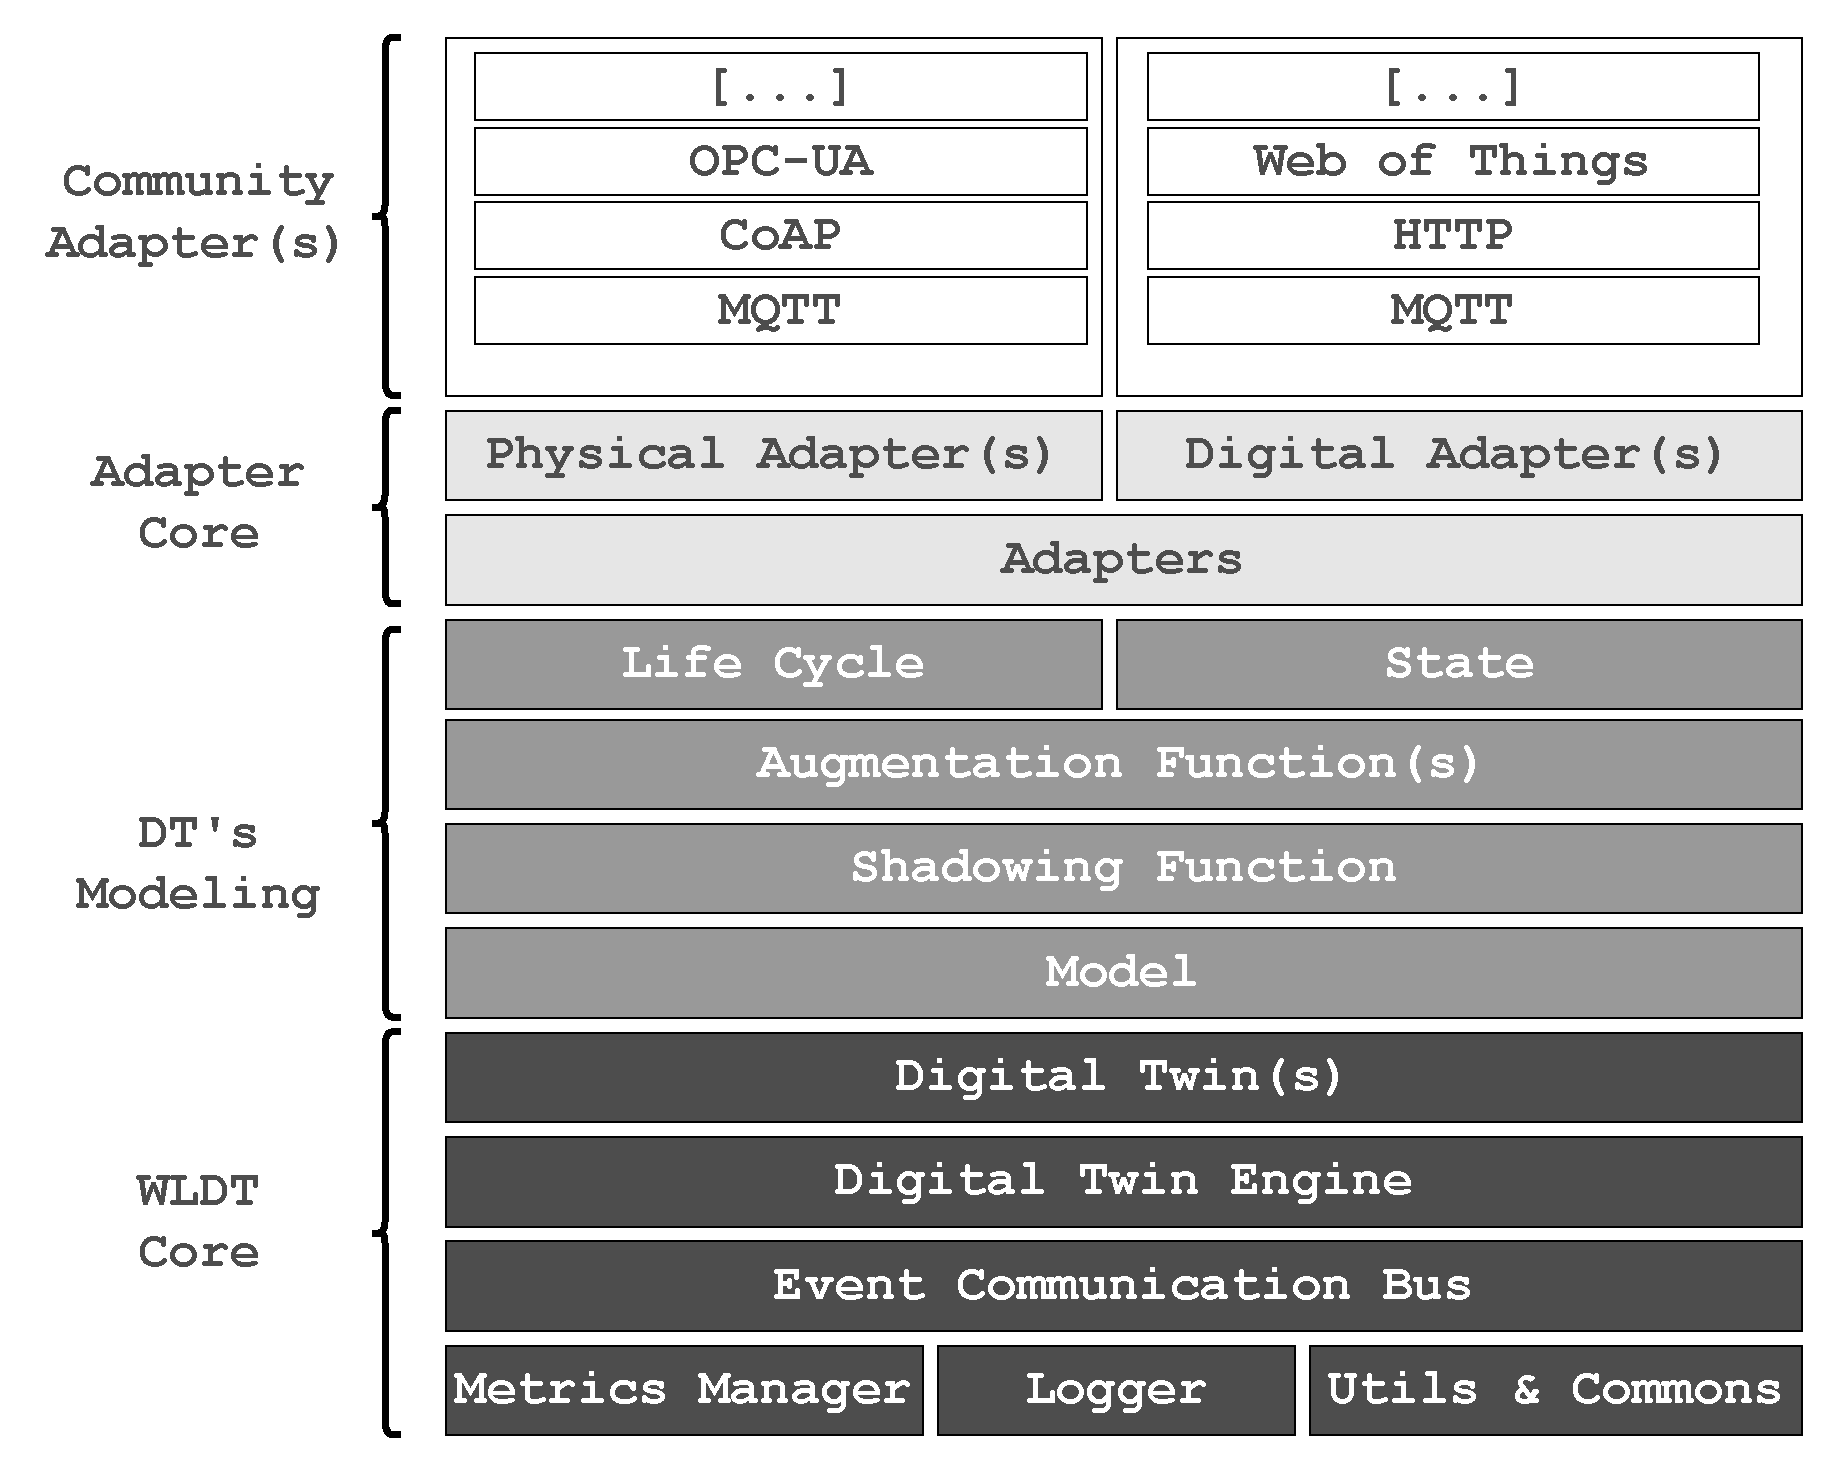
\includegraphics[width=\columnwidth]{figures/engineering-wldt/wldt_architecture.pdf}
    \caption{WLDT Framework's Software Architecture.}
    \label{fig:wldt_architecture}
\end{figure}

This abstract structure defines the foundational building blocks implemented in the WLDT framework. The DTM captures and represents the PT at the desired level of abstraction, modeling only domain-level information rather than technological details~\cite{dt-IoT-context-Minerva-2020}.
The shadowing process enables continuous and near-real-time updating of the DT's State (DTS) characterized by: i) \textit{Properties:} Observable attributes of the corresponding PT, represented as labeled data whose values can dynamically change over time, in accordance with the PT's state evolution;
ii) \textit{Events:} Domain-level occurrences that can be observed in the PT;
iii) \textit{Relationships:} Links between the modeled PT and other physical assets within the organization through their corresponding DTs. Relationships can be dynamically created and modified over time, reflecting the operational context rather than the PT's state;
and iv) \textit{Actions:} Operations that can be invoked on the PT through interaction with the DT or directly on the DT if not available on the PT, thereby augmenting the PT's physical capabilities.
When actions are invoked, the DT receives an action request on its DI, applies the shadowing function to validate it, and then may propagate the request through its physical interface and the associated PT.
It is crucial to note that a digital action request does not directly change the state of the DT.
Any changes occur only as a result of the shadowing function from the PT to the DT, as previously described. 

% It is worth pointing out that the digitalization process of the physical entity within the DT follows the shadowing principle defined in~\cite{DT-in-manufacturing-review-Kritzinger-2018} but is not limited to it, as the DTM also takes into account interactions coming from the digital space.
%Therefore, the correspondence between the proposed framework's modelling and the envisioned approach in the state of the art is respected.

\begin{figure}[t]
    \setlength{\belowcaptionskip}{-13pt}
    \centering
    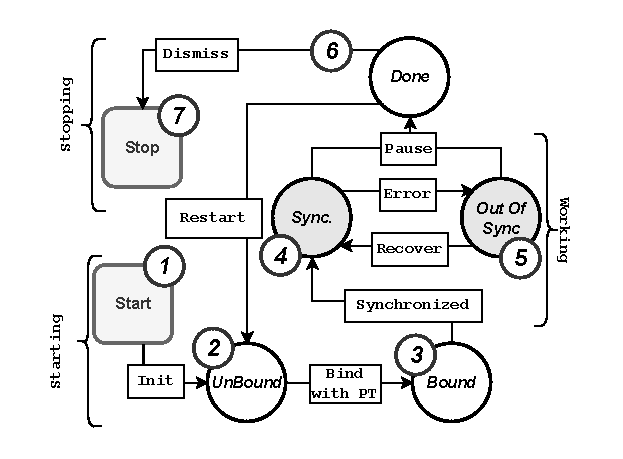
\includegraphics[width=\columnwidth]{figures/engineering-wldt/wldt_lifecycle_simple.pdf}
    \caption{DT Life Cycle in WLDT with its phases and transitions.}
    \label{fig:wldt_life_cycle}
\end{figure}

Augmentation functions enhance a DT’s capabilities beyond simple replication of the PT, enabling added functionalities and behaviors not directly observable or executable by the PT. They operate in close interaction with the DTS—capturing the PT’s real-time properties, events, relationships, and actions—and the model, which defines the logic governing these elements. By leveraging the model, augmentation functions interpret DTS changes to enable advanced analytics, predictive maintenance, and informed decision-making. In doing so, they transform raw state data into actionable insights, adding significant value to the DT.

%% BEFORE CAMERA READY
% The augmentation functions play a critical role in enhancing the capabilities of a DT beyond merely replicating the PT.
% They allow the DT to incorporate additional functionalities and behaviors that may not be directly observable or executable by the PT itself.
% These functions interact closely with the DTS and DTM.
% The DTS encapsulates the current properties, events, relationships, and actions that reflect the real-time status and interactions of the PT.
% The model, on the other hand, defines the rules, logic, and behavior governing how these state elements are managed and manipulated.

% The augmentation function leverages the model to interpret and respond to changes in the DTS, enabling the DT to perform advanced analytics, predictive maintenance, and other complex operations that are informed by, but not limited to, the PT's data. It ensures that the DT not only mirrors the physical entity but also provides added value through enhanced data processing, decision-making capabilities, and actionable insights.
% Thus, the augmentation function serves as a bridge that transforms raw state information into meaningful, actionable outcomes guided by the underlying model.



\subsection{WLDT: A New Plugin-Based Architecture} 
\label{sec:wldt-architecture}

The WLDT framework has been re-designed and extended with key requirements: \textit{Simplicity}, \textit{Extensibility}, \textit{Portability}, and \textit{Microservice Readiness}.
Simplicity ensures easy creation of DT instances using existing modules or custom behaviors for specific scenarios. 
Extensibility allows easy API extension, enabling customization and addition of new features through concurrent module execution.
Portability and microservice readiness ensure that DTs can run on any platform without modifications.
The core engine is lightweight, offering IoT features for developing DT applications as independent microservices.
The main components of the WLDT architecture are illustrated in Figure~\ref{fig:wldt_architecture}, which outlines the three architectural levels: the core library, the DT model, and the implementation of physical and digital interfaces through adapters.
In the WLDT framework, \textit{adapters} -- modular components that implement the PI and DI -- are essential for facilitating communication between PTs and DTs, as well as with external digital entities.
Physical Adapters (PAs) interface with the physical world, while Digital Adapters (DAs) manage interactions within the digital environment.

The \textit{Metrics Manager} provides the functionalities for managing and tracking various metrics within DT instances, combining both internal and custom metrics through a flexible and extensible approach.
The \textit{Logger} is designed to facilitate efficient and customizable logging within implemented and deployed DTs, with configurable log levels and versatile output options.
The \textit{Utils \& Commons} component contains a collection of utility classes and common functionalities that can be readily employed across DT implementations, ranging from handling common data structures to providing helpful tools for string manipulation.

%%%
\begin{figure}[th!]
    \setlength{\belowcaptionskip}{-8pt}
    \centering
    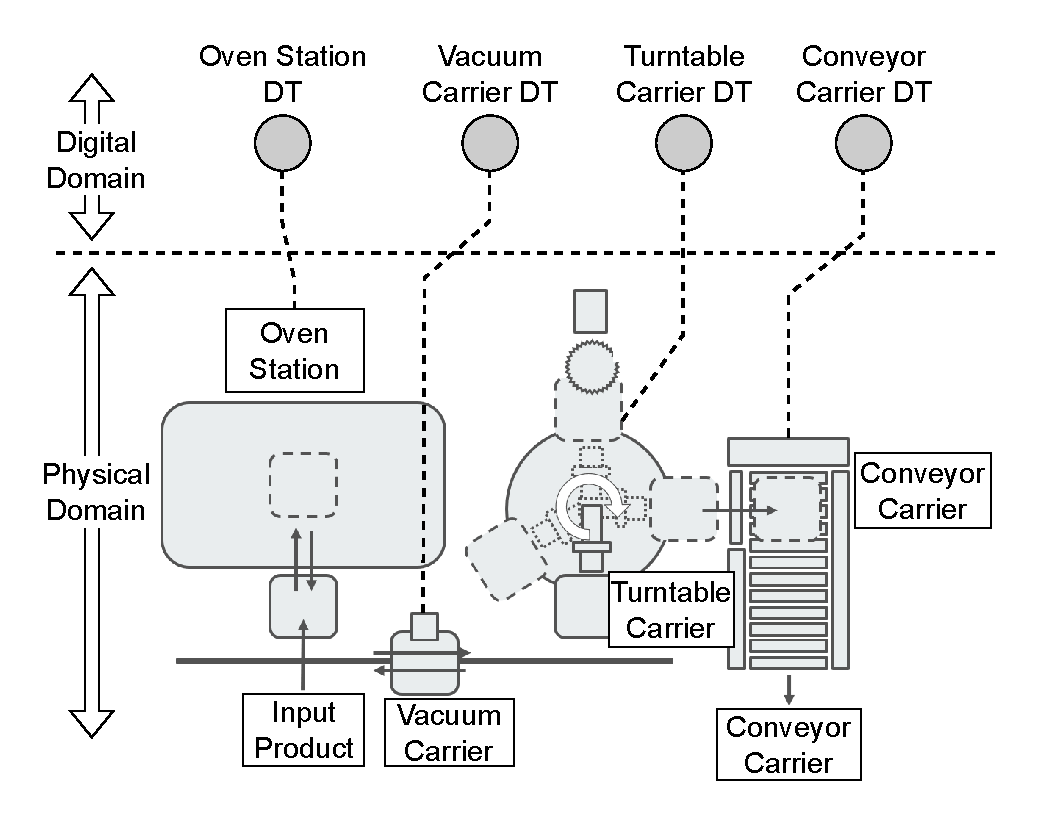
\includegraphics[width=\columnwidth]{figures/engineering-wldt/fischer-layout-first-level-dt.pdf}
    \caption{A schematic view of the target industrial scenario.}
    \label{fig:discher-dt-first-level}
\end{figure}
%%%

The \textit{Event Communication Bus} represents the internal Event Bus, designed to support communication between the different components of the DT instance (PI, DTM and DI). It allows for the definition of customized events to model both physical and digital inputs and outputs. Each WLDT component can publish on the shared Event Bus and define an Event Filter to specify which types of events it is interested in managing, associating a specific callback to process different messages.

%%%
\begin{figure*}[th!]
    \setlength{\belowcaptionskip}{-13pt}
    \centering
    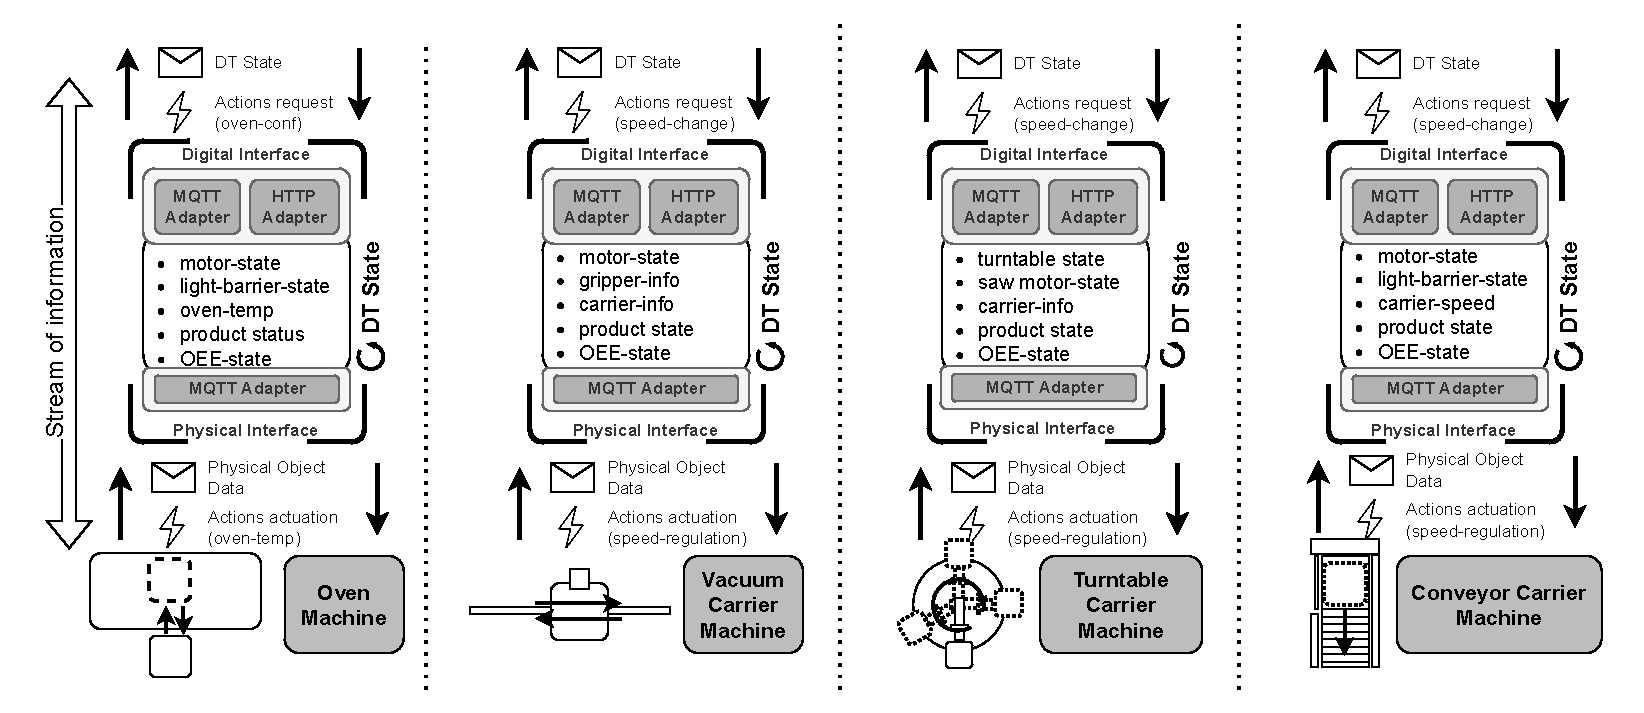
\includegraphics[width=0.95\textwidth]{figures/engineering-wldt/DTs-zoom-in.pdf}
    \caption{Internal structure of machine-level DTs with the details of adapters, states and capabilities}
    \label{fig:dt-internal-structure-overview}
\end{figure*}
%%%

The \textit{Digital Twin Engine} defines the multi-threaded engine of the library, allowing the execution and monitoring of multiple DTs and their core components simultaneously.
It orchestrates the different internal modules of the architecture while keeping track of each one, and it serves as the core of the platform, enabling the execution and control of deployed DTs.
Currently, it supports the execution of twins within the same Java process, but the same engine abstraction could extend the framework to support distributed execution through different processes or microservices.

The DT component consists of a modular structure within WLDT, combining core functionalities and capabilities of physical and digital adapters.
Each DT's core module is its \textit{Model}, which is responsible for implementing the twin's behavior over time. This model controls both the \textit{Shadowing Function} and \textit{Augmentation Function(s)}.
The Shadowing Function manages the digitalization process by integrating data from physical adapters and action requests from digital adapters.
It maintains the DT's \textit{State}, organizing properties, events, actions, and relationships as introduced in Section \ref{sec:dt_modelling}.
Augmentation Functions enhance physical capabilities by introducing new properties and actions through intelligent functionalities or dedicated processing (e.g., anomaly detection or data aggregation).
The DT's core is managed by the library to ensure consistency and lifecycle management, adapting to computational phases and interactions with physical and digital realms via adapters. 
Further sections elaborate on these aspects concerning lifecycle structure and adapters.

%%%
\subsection{Cyber-Physical Awareness \& Life-cycle}
\label{sec:dt-lifecycle}

The modeling of DTs involves defining their life cycle, which we have mapped into five states: \textit{UnBound}, \textit{Bound}, \textit{Synchronized}, \textit{OutofSync}, and \textit{Done}.
These states are directly inspired by recent state-of-the-art definitions in the field, particularly from \cite{web_of_dt} and \cite{bellavista2023requirements}, which provide a comprehensive framework for understanding and managing the dynamic evolution of DTs across different stages.

In the \textit{UnBound} state, all internal modules are active but not yet associated with the corresponding PT.
The DT transitions to the \textit{Bound} state once the binding procedure is completed, establishing a connection with the PT and enabling bidirectional event flow.
In the \textit{Synchronized} state, the DT’s state is aligned with the PT, initiating the shadowing process.
The \textit{OutofSync} state indicates errors in the shadowing process, where state alignment or application-generated events cannot be processed.
Finally, the DT reaches the \textit{Done} state when the shadowing process ends but remains active for external requests (e.g., asset history access after its lifecycle).

To transition from \textit{UnBound} to \textit{Bound}, the DT establishes a relationship with the Physical Layer.
For instance, a PT using two protocols, $P_1$ and $P_2$, communicates through dedicated adapters.
A key challenge is discovering the PT’s capabilities to begin the digitalization process. WLDT addresses this by describing a PT’s characteristics, properties and actions through its physical adapters enabling the DT to synchronize with the PT.
The DT transitions to \textit{Bound} only when the required adapters are bound and PT descriptions are generated, even when multiple PTs are associated with a single DT.

To move from \textit{Bound} to \textit{Synchronized}, the DT identifies PT capabilities for digitalization and starts the shadowing process (e.g., monitoring a thermostat's target temperature and humidity sensors).
The DT’s Model begins observing these properties through the adapters, which communicate with the PT and generate events for property changes.
The DT’s Shadowing function processes these events to compute the new DT state, maintaining synchronization with the PT.
Any change in the DT state generates an event, which is exposed to the digital world through the Digital Interface and its Adapters.
These events may also trigger actions on the DT or propagate requests to the PT if needed.

%%%
\subsection{Modular and Reusable Digital \& Physical Adapters}
\label{subsec:adapters}

A Physical Adater (PA) in WLDT is responsible for connecting to a specific PT. 
Developers can either leverage existing adapters—customized through configuration for context-specific reuse—or create new ones tailored to their specific requirements.
The core responsibilities of a PA include also the generation of a description of the associated PT that details the properties, events, actions, and relationships of the PT; producing events to reflect changes in the physical state, such as variations in properties, events, and relationships; and handling action requests from the digital realm via the DT shadowing function and the twin's model.
Each PA has an internal dedicated lifecycle within the DT to ensure it can respond to incoming actions appropriately. Adapters are identified by unique IDs, enabling the library to coordinate multiple adapters, adjust logs, and execute functions upon receiving new events. 

Conversely, Digital Adapters (DAs) in WLDT act as the bridge between the DT's core and the external digital world.
Their primary functions include receiving and exposing events related to changes in properties, events, available actions, and relationships from the DT’s core;
communicating the received information to external systems according to the implementation and supported protocols;
and handling incoming digital actions, forwarding them to the core, and ensuring they are validated and processed by the Shadowing Function.
Each DA has an internal life cycle to support its coordination by the WLDT core and has also direct read access to the current twin's State through callbacks or synchronous access, allowing it to navigate all fields of the current digital state and expose it in the digital domain through various protocols according to the application context.


%========================================================
\section{Benefits of the Proposed Approach}
%========================================================

\subsection{Interoperability in a Manufacturing Use Case}
\label{sec:industrial_use_case}
%%%

%%%
\begin{figure*}[t]
    \setlength{\belowcaptionskip}{-13pt}
    \centering
    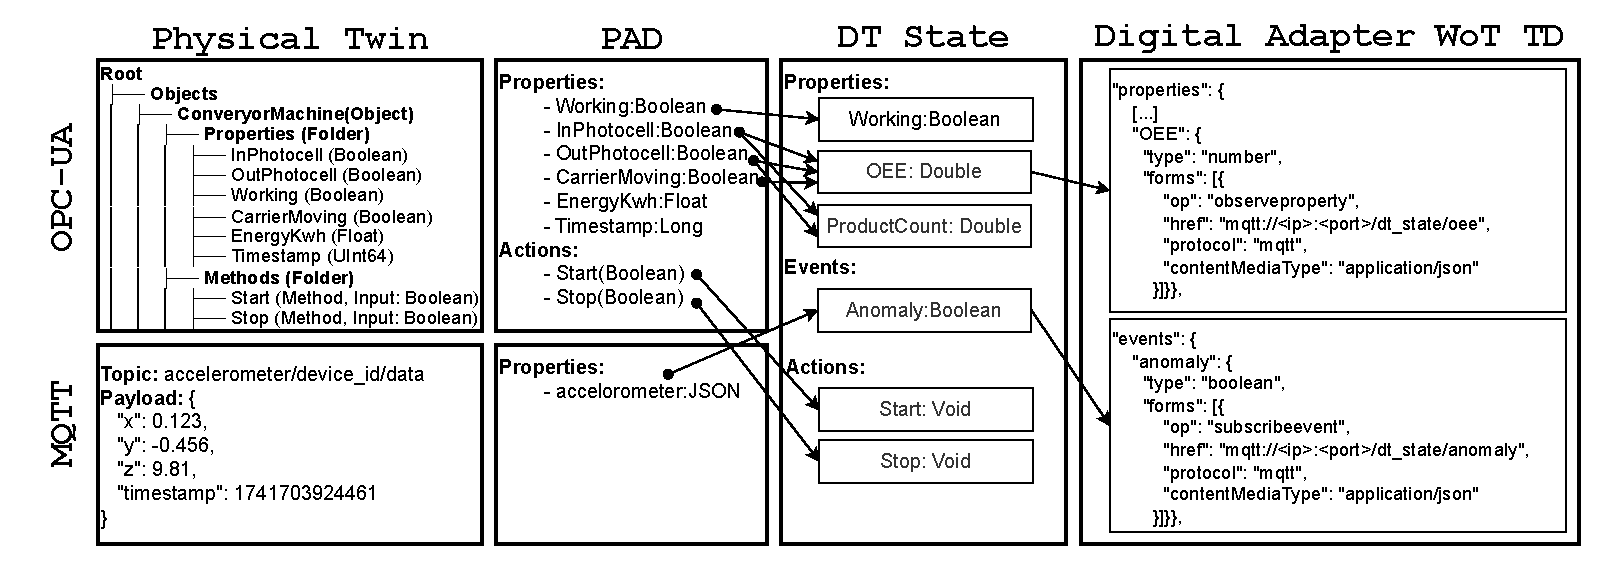
\includegraphics[width=\textwidth]{figures/dt-interoperability/dt_interoperability-pad_dt_wot.pdf}
    \caption{The transition from physical to digital representation via the \ac{PAD}, the \ac{DT} State, and the \ac{DTD} for external consumers.}
    \label{fig:pad_dt_wot}
\end{figure*}
%%%

The proposed \ac{DT} architectural approach is showcased using the \emph{Fischertechnik Training Factory Industry 4.0}\footnote{Fischertechnik Industry \& Universities: \url{https://www.fischertechnik.de/en/products/industry-and-universities}} Indexed-Line Station, controlled by a Siemens PLC that publishes real-time data via OPC-UA, integrated with Arduino RP2040 boards\footnote{Arduino RP2040: \url{https://docs.arduino.cc/hardware/nano-rp2040-connect/}} for accelerometer data collection and processing and communicating over MQTT\footnote{MQTT Protocol: \url{https://mqtt.org/}}.

\begin{figure}[ht]
  \setlength{\belowcaptionskip}{-5pt}
  \centering
  \begin{subfigure}[t]{0.32\linewidth}
      \centering
      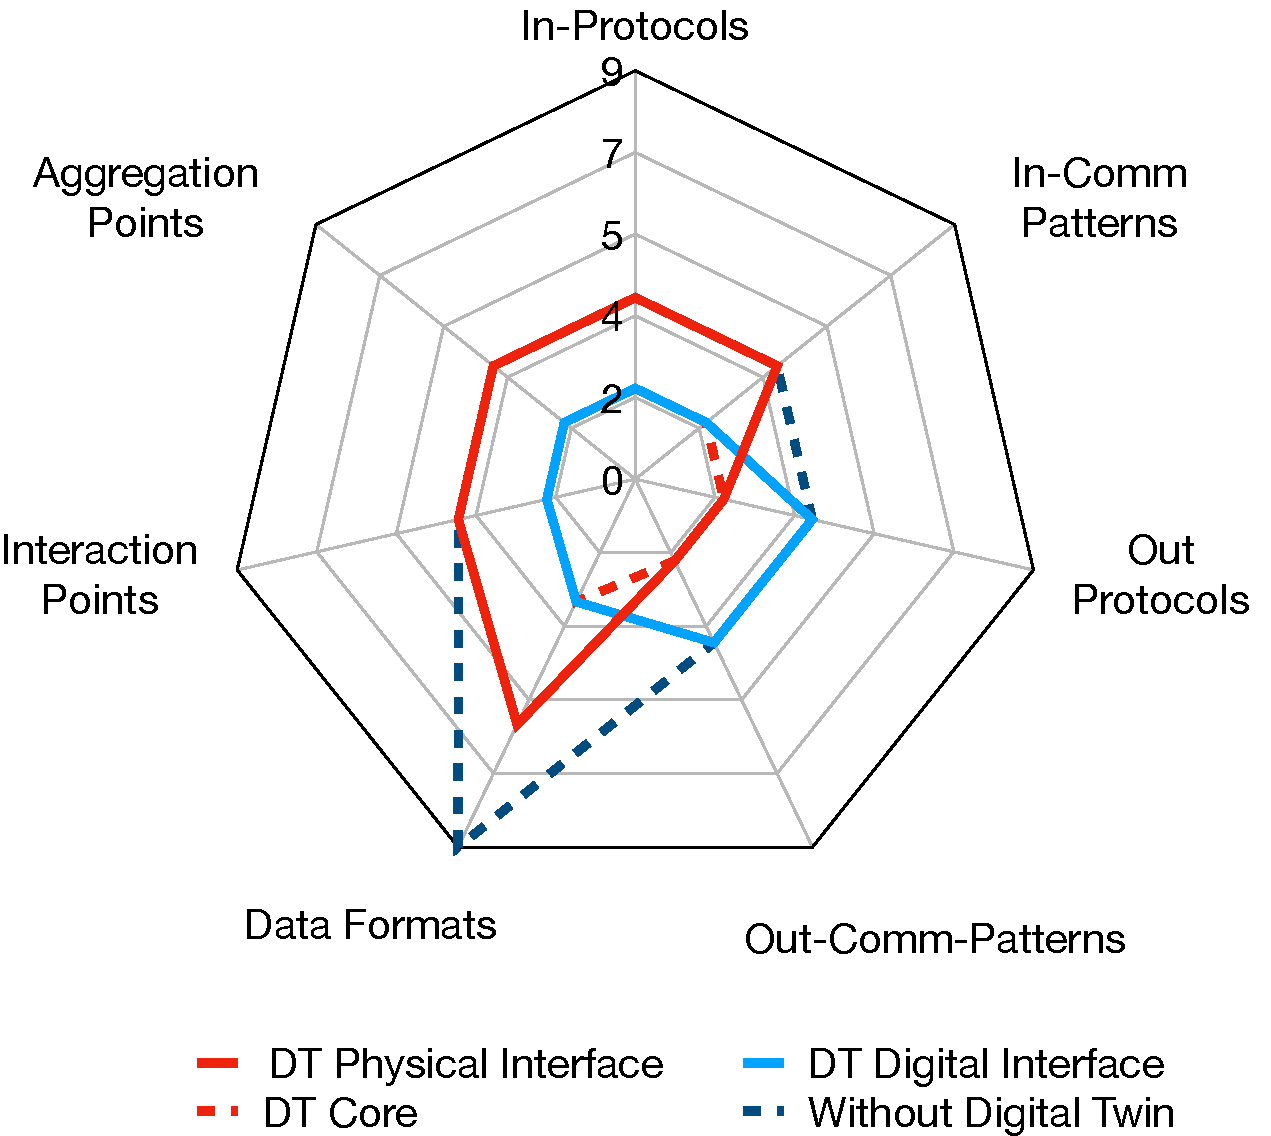
\includegraphics[width=\linewidth]{figures/dt-interoperability/machine_complexity_index.pdf}
      \caption{Machine Digital Twin}
      \label{fig:machine_complexity_index}
  \end{subfigure}
  \begin{subfigure}[t]{0.32\linewidth}
      \centering
      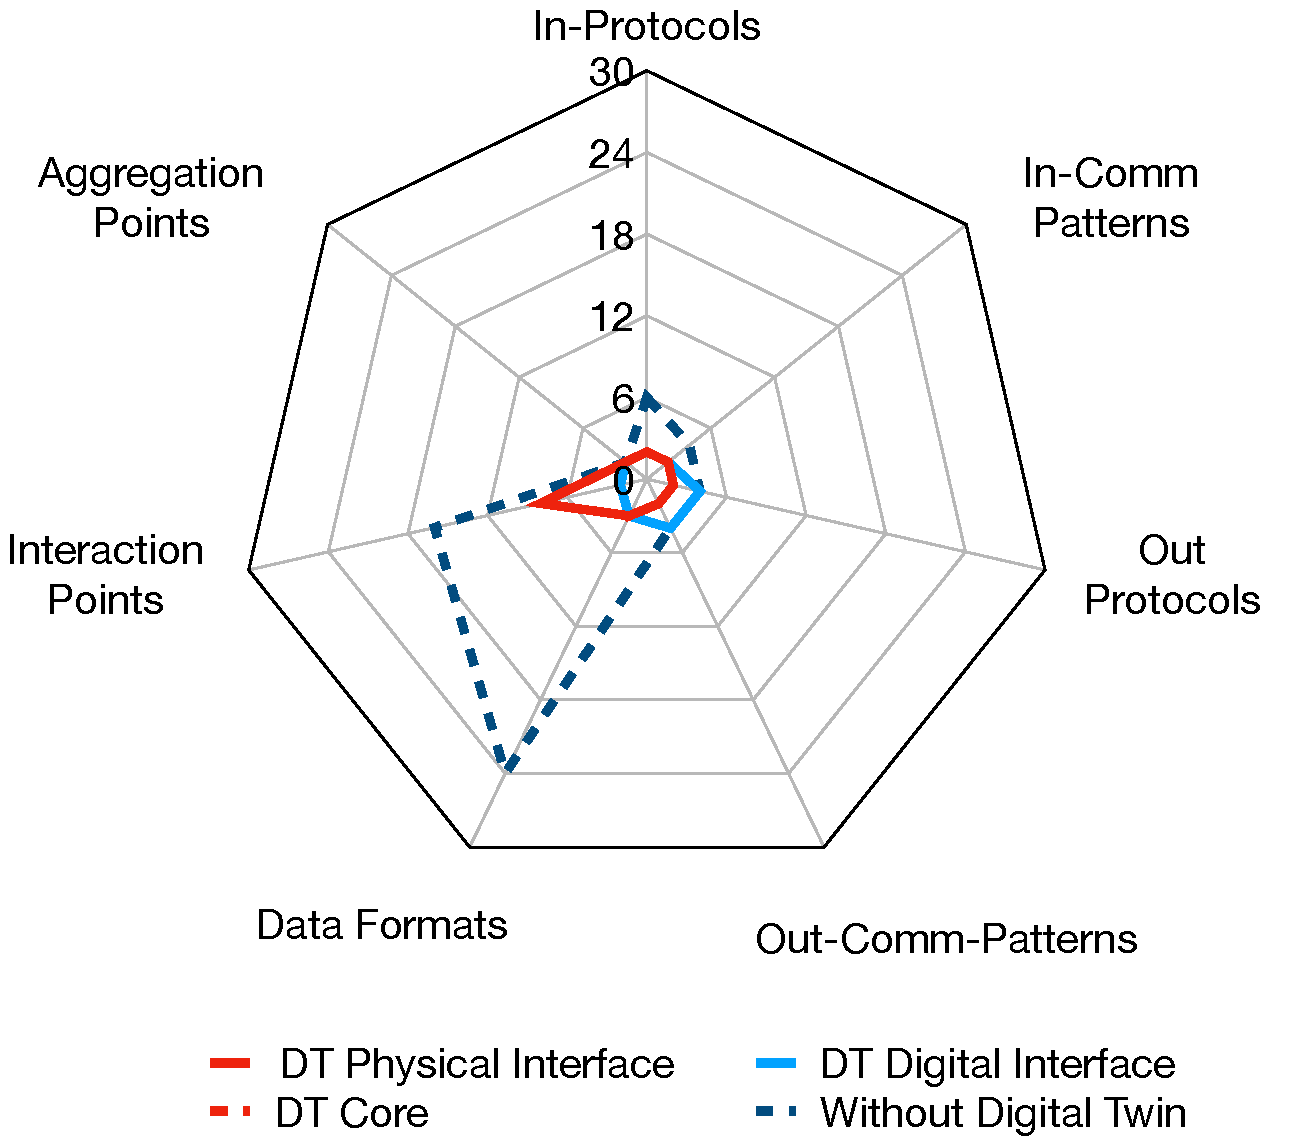
\includegraphics[width=\linewidth]{figures/dt-interoperability/station_complexity_index.pdf}
      \caption{Station (Indexed-Line) Digital Twin}
      \label{fig:station_complexity_index}
  \end{subfigure}
  \begin{subfigure}[t]{0.32\linewidth}
      \centering
      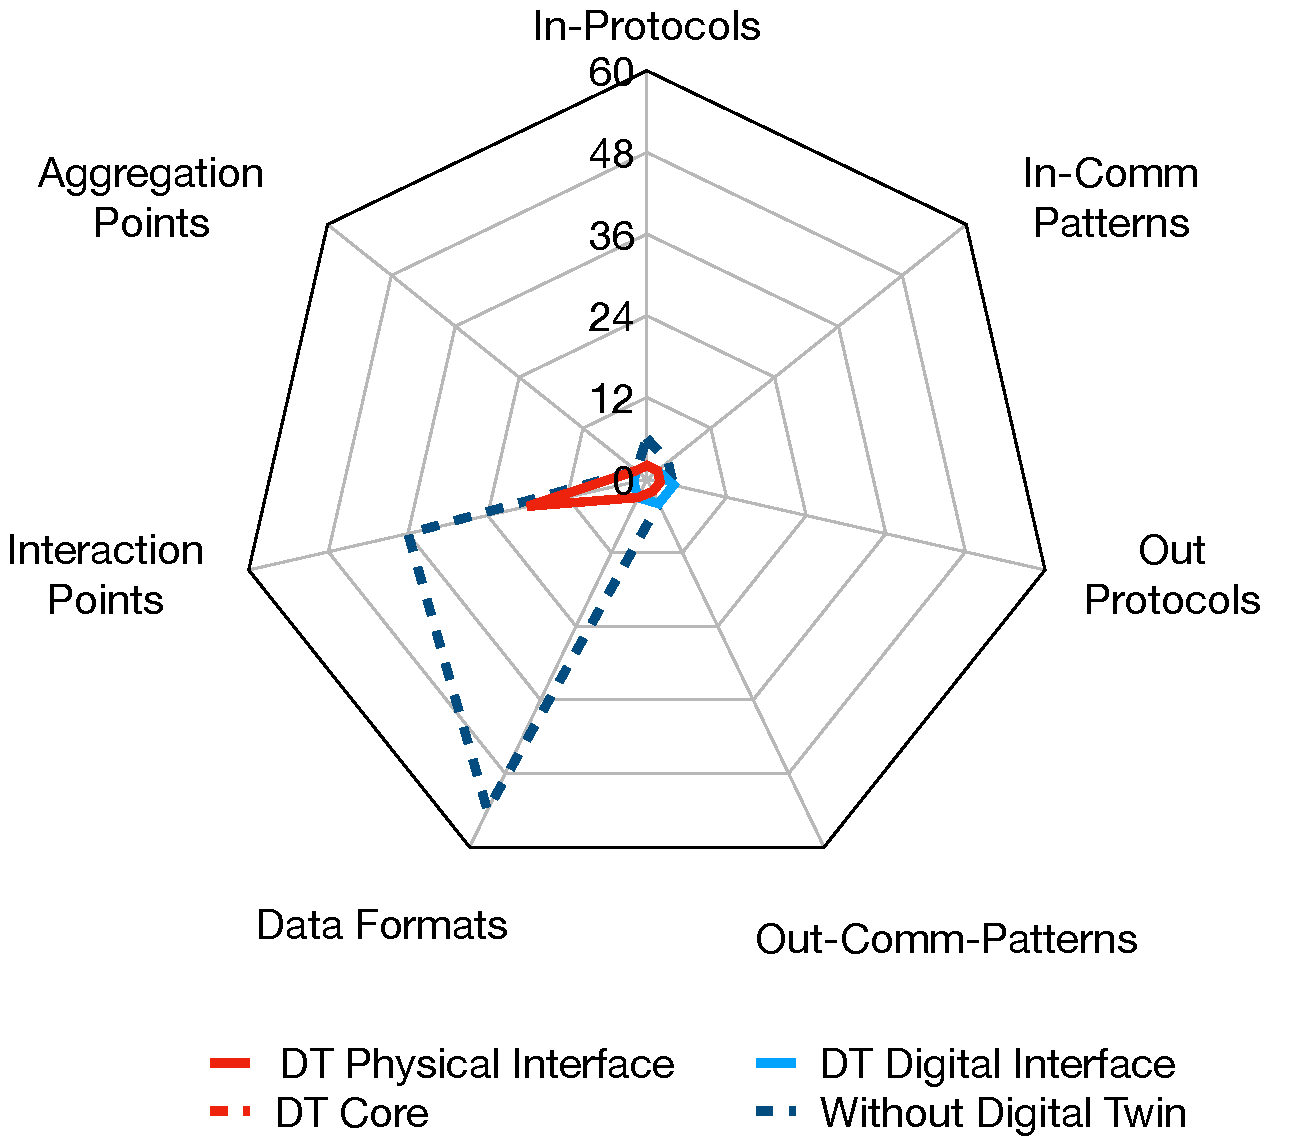
\includegraphics[width=\linewidth]{figures/dt-interoperability/factory_complexity_index.pdf}
      \caption{Factory Digital Twin}
      \label{fig:factory_complexity_index}
  \end{subfigure}
  \caption{Schematic representation of cyber-physical complexity and its impact on various components.}
  \label{fig:dt_complexity_index}
\end{figure}

The scenario emulates a production line, with a \ac{DT} system deployed to monitor production and measuring the overall efficiency.
The \ac{DT} ecosystem architecture is depicted in Figure \ref{fig:mf_dt_ecosystem}.
Four machine-level \acp{DT} are deployed, each with a \ac{PI} supporting the relevant communication protocols to interact with the different machines, namely through MQTT and OPC-UA\footnote{OPC-UA: \url{https://opcfoundation.org/about/opc-technologies/opc-ua/}}.
These \acp{DT} track machine states, monitor performance, and coordinate production by processing data from the physical system and digital action requests.
An additional department-level \ac{DT} aggregates data from machine-level \acp{DT}, extracting system metrics and exposing department-level actions. 

All the \acp{DT} are built using the \ac{WLDT} open-source framework\footnote{WLDT framework: \url{https://wldt.github.io}}: a Java-based multithreaded stack, facilitating the definition of \ac{DT} and supporting the implementation of shadowing and digitalisation processes.
%Within the framework, we implemented our proposal of physical and digital adapters to validate the approach and facilitate interoperability with a broader range of devices and applications.
The frameworks implements our proposal of physical and digital adapters that we exercise in this example.

\ac{DT} of composed physical assets, such as the \textit{Indexed Line Department} \ac{DT} (see Figure \ref{fig:mf_dt_ecosystem}, top) use lower-level \acp{DT} as data sources.
Notably, the physical and digital adapters that implement MQTT, OPC-UA, and HTTP protocols, along with \ac{WoT} over HTTP for serving \acp{TD}, are reusable across different instances.
These adapters, through configurable parameters, enable effective communication and integration within both digital and physical environments.

Machine-level \acp{DT} provide real-time data on their physical counterparts, such as workpiece presence, operational state
(e.g., idle, working, waiting, or broken),
and performance KPIs like \ac{OEE}\footnote{OEE: \url{https://www.oee.com/}}, calculated from production rate, uptime, and downtime.
%
At the department level, \acp{DT} representing the Indexed Departments assess performance by computing Weighted \ac{OEE}~\cite{OEE-manufacturing-cell-Gamberini-2017,Introduction-to-TPM-total-productive-maintenance-Nakajima-1995}, derived from individual machine \acp{DT}, and track throughput, defined as processed pieces per unit time.
Throughput is determined by monitoring entry and exit events within the department, utilizing relationships captured by the associated \acp{DT}.

Upon startup, each \ac{DT} connects to its data source, publishes the \ac{PAD} of the physical asset, and interacts with the PLC or Arduino to collect and send data, enabling digitalization and interoperability among heterogeneous equipment. 

Figure \ref{fig:pad_dt_wot} schematically illustrates the evolution of data and representation from the physical to the digital realms through the adoption of the proposed \ac{DT} architectural approach, \ac{PAD} integration, and \ac{WoT} \acp{TD} used as \acp{DTD} on the digital side, specifically for the output conveyor of the target production line.
On the physical side, data is structured using OPC-UA with a hierarchical organization, containing telemetry data and action methods mapped to specific data types.
Accelerometer data is transmitted over MQTT on a specific topic with a JSON payload containing axis acceleration values. 

The \acp{PAD} act as an intermediary, translating data from the PT into a format suitable for the DT core, decoupling it from the complexity of interacting with the \ac{PT} and enabling discovery, understanding, and utilization of available data and methods.
Using the information from the \acp{PAD}, the \ac{DT} model computes the \ac{DT}'s state with target properties, events, and actions, based on either one-to-one matching of physical characteristics or augmented by combining multiple physical properties into computed \ac{DT} properties or events, such as computing the value of the \ac{OEE} property or triggering anomaly detection events based on accelerometer data. 

Finally, the \ac{DiA} of the \ac{DT} leverages \ac{WoT} \ac{TD} to describe the DT's data and functionalities through a standardized, interoperable, and machine-readable approach.
The \ac{TD} specifies how these can be accessed via protocols and data formats.
This approach enables effective interoperability from the physical to the digital, using a modular and decoupled structure through \acp{DT} in the target industrial use case.

\subsection{Mapping Cyber-Physical Complexity}
\label{sec:mappint_cp_complexity}

In our experimental analysis, we also aim to measure the impact of digitization and responsibility decoupling by comparing the system complexity in scenarios with and without \ac{DT} adoption and also with respect to the different \ac{DT}'s architectural layers.
This allows us to assess the benefits of a modular, structured DT-based approach, particularly in terms of interoperability and heterogeneity management.
To quantify how effectively our approach manages cyber-physical heterogeneity, we adopt the \textit{Cyber-Physical Complexity Index (CP-CI)} proposed in \cite{lippi_dt_causality_learning, LOMBARDO2024107203}.
The CP-CI quantifies the complexity of a cyber-physical application based on:
i) \textit{Required Protocols (p)}: communication protocols needed for device interaction;
ii) \textit{Communication Patterns (c)}: interaction models (e.g., Publish/Subscribe, Request/Response);
iii) \textit{Data Formats (d)}: required data representations or serialization methods;
iv) \textit{Interaction Points (n)}: modules or services involved in data exchange; and
v) \textit{Aggregation Points (a)}: levels of abstraction for physical data (e.g., merging data from multiple machines).
Each criterion is weighted with a \textit{Criteria Importance Factor ($CIF$)} from 1 (low) to 3 (high), indicating its impact on development, deployment, and maintenance.

% The CP-CI reflects the perceived complexity of a cyber-physical application, based on the following criteria: i) \textit{Required Protocols (p)}: number of communication protocols needed to interact with physical devices; ii) \textit{Communication Patterns (c)}: number of interaction models (e.g., Publish/Subscribe, Request/Response); iii) \textit{Data Formats (d)}: number of data representations or serialization methods required; iv) \textit{Interaction Points (n)}: number of distinct modules or services involved in data exchange; and v) \textit{Aggregation Points (a)}: number of composition levels needed to abstract physical information (e.g., merging data from multiple machines in a line). Each criterion is weighted using a \textit{Criteria Importance Factor ($CIF$)}, ranging from 1 (low) to 3 (high), to reflect its impact on development, deployment, and system maintenance.

Focusing on \ac{DT} interoperability, we extended the CP-CI to include both inbound and outbound interfaces, essential for bridging the physical and cyber layers with differing requirements.
This extension enables a more precise assessment of the complexity in managing interoperability across system boundaries.
The CP-CI was applied not only to the entire \ac{DT} but also to its internal layers: Physical Interface (PI), Core, and Digital Interface (DI).
These results were compared to those of a monolithic external application that directly handles business logic and interoperability, bearing the full complexity, highlighting the advantages of the modular \ac{DT} design.
High importance ($CIF=3$) was assigned to managing heterogeneous data formats ($d$) and aggregation points ($a$), as they are crucial for creating interoperable data models.
Medium importance ($CIF=2$) was given to protocol diversity ($p$) and interaction with multiple entities ($n$), which become more significant as systems scale.
Low importance ($CIF=1$) was assigned to multiple communication patterns ($c$), as their concurrent use is standard in distributed applications.

The graphs presented in Figure \ref{fig:dt_complexity_index} display the CP-CI values obtained across different levels of deployment: a single machine, a station in the factory (such as the indexed line, where multiple machines and their respective DTs are managed and composed into a single, unified DT), and the entire factory, which includes 9 machines, 2 composed DTs, and one overarching DT for the entire factory, all deployed following the proposed modular and interoperable approach.
For the machines analyzed, the involved protocols ($p$) and communication patterns ($c$) are both set to 2, as we utilize MQTT and OPC-UA with Pub/Sub and Request/Response interactions.
On the digital side, both MQTT and HTTP are employed.
Regarding data formats ($d$), each machine manages 2 distinct formats, accounting for both PLC data and Arduino accelerometer information.
Furthermore, the interaction points ($n$) and aggregation points ($a$) are both 2, reflecting the aggregation and interaction with two different sub-entities for each machine and its corresponding DT.

The results for single machines (Figure \ref{fig:machine_complexity_index}) highlight the critical role of the PI in the \ac{DT} architecture.
As a decoupling layer, the PI isolates physical-world complexities from the DT core, managing priorities like protocols, data formats, interaction points, aggregation strategies, and communication patterns.
This allows the DT core to focus on uniform data, processed through the interface via PAD descriptions and payload transformations, without dealing with heterogeneous physical entities.
Consequently, the core interacts only with its internal communication pattern and consistent interaction points, regardless of the physical environment’s configuration.
A similar approach is applied to the DI, which is decoupled from physical complexities and adapts to external digital systems, ensuring modularity and reuse.

In contrast, systems without a \ac{DT} must embed all heterogeneity management into a single application, burdening it with business logic, protocol diversity, and data format interoperability.
This increases complexity and reduces scalability, as reflected by the complexity index parameters.

% The results for single machines (reported in Figure \ref{fig:machine_complexity_index}) underscore the strategic importance of the PI within the \ac{DT} architecture. Acting as a decoupling layer, the PI isolates the complexities of the physical world from the DT core. It manages key priorities related to the physical domain, including protocols, data formats, interaction points, aggregation strategies, and communication patterns. This separation allows the DT core to focus on uniform data, processed and normalized through the interface using PAD descriptions and payload transformations, rather than managing heterogeneous physical entities. As a result, the DT core is shielded from the diversity of protocols, working only with its internal communication pattern and a consistent set of interaction points, regardless of the physical environment's configuration. A similar approach applies to the DI, which is decoupled from physical-world complexities and its interaction is limited to the DT core, adapting to external digital systems based on the specific application context. This modular approach enhances the separation of concerns and promotes reuse, allowing the same DT core to be deployed with various Physical Interfaces suited to different operational contexts.

% In contrast, systems that lack a \ac{DT} approach, which bridges and manages the cyber-physical layers, must integrate all interoperability and heterogeneity management into a single application. This places the burden of handling business logic, protocol diversity, and data format interoperability on the application itself, leading to increased complexity and diminished scalability, as reflected in the parameters of the complexity index.

As system architecture scales from individual machines to stations, production lines (Figure \ref{fig:station_complexity_index}), or entire factories (Figure \ref{fig:factory_complexity_index}), protocol diversity stabilizes while the number of interaction points and data formats increases due to the need for managing heterogeneous components.
Our complexity measure shows that systems at the station or factory level experience a significant rise in complexity, driven by interaction points, aggregation nodes, and data format diversity.
These results emphasize the benefits of a modular and interoperable approach.
By encapsulating complexity within DT modules and using interoperable representations, developers can simplify application development.
In contrast, monolithic systems struggle with managing interoperability and system evolution as integration requirements grow.


\subsection{Industrial Use Case}
\label{sec:industrial_use_case}
%To demonstrate the applicability of the proposed lifecycle synchronization model, we conducted an experimental evaluation within a real-world industrial scenario. This evaluation highlights how the alignment between the DT and PT lifecycles can be effectively achieved through structured data management and phase synchronization. The industrial case involves mapping the lifecycle phases of physical devices.

An industrial scenario has been considered to apply the proposed approach for DT's lifecycle modeling and characterization. Specifically, scaled industrial stations manufactured by Fischertechnik\footnote{Fischertechnik: \url{https://www.fischertechnik.de/en/products/industry-and-universities}} has been adopted as reference industrial prototyping environment with multiple stations and involved machines. The first station, referred to as the \textit{Multiprocess Station with Oven}, features an oven, a robotic arm for handling operations, and a rotary table equipped with multiple processing stages. The second station, named the \textit{Indexed Line}, comprises four conveyor belts, two of which include mechanical processing operations for the workpieces.

\begin{figure}[ht]
    \setlength{\belowcaptionskip}{-13pt}
    \centering
    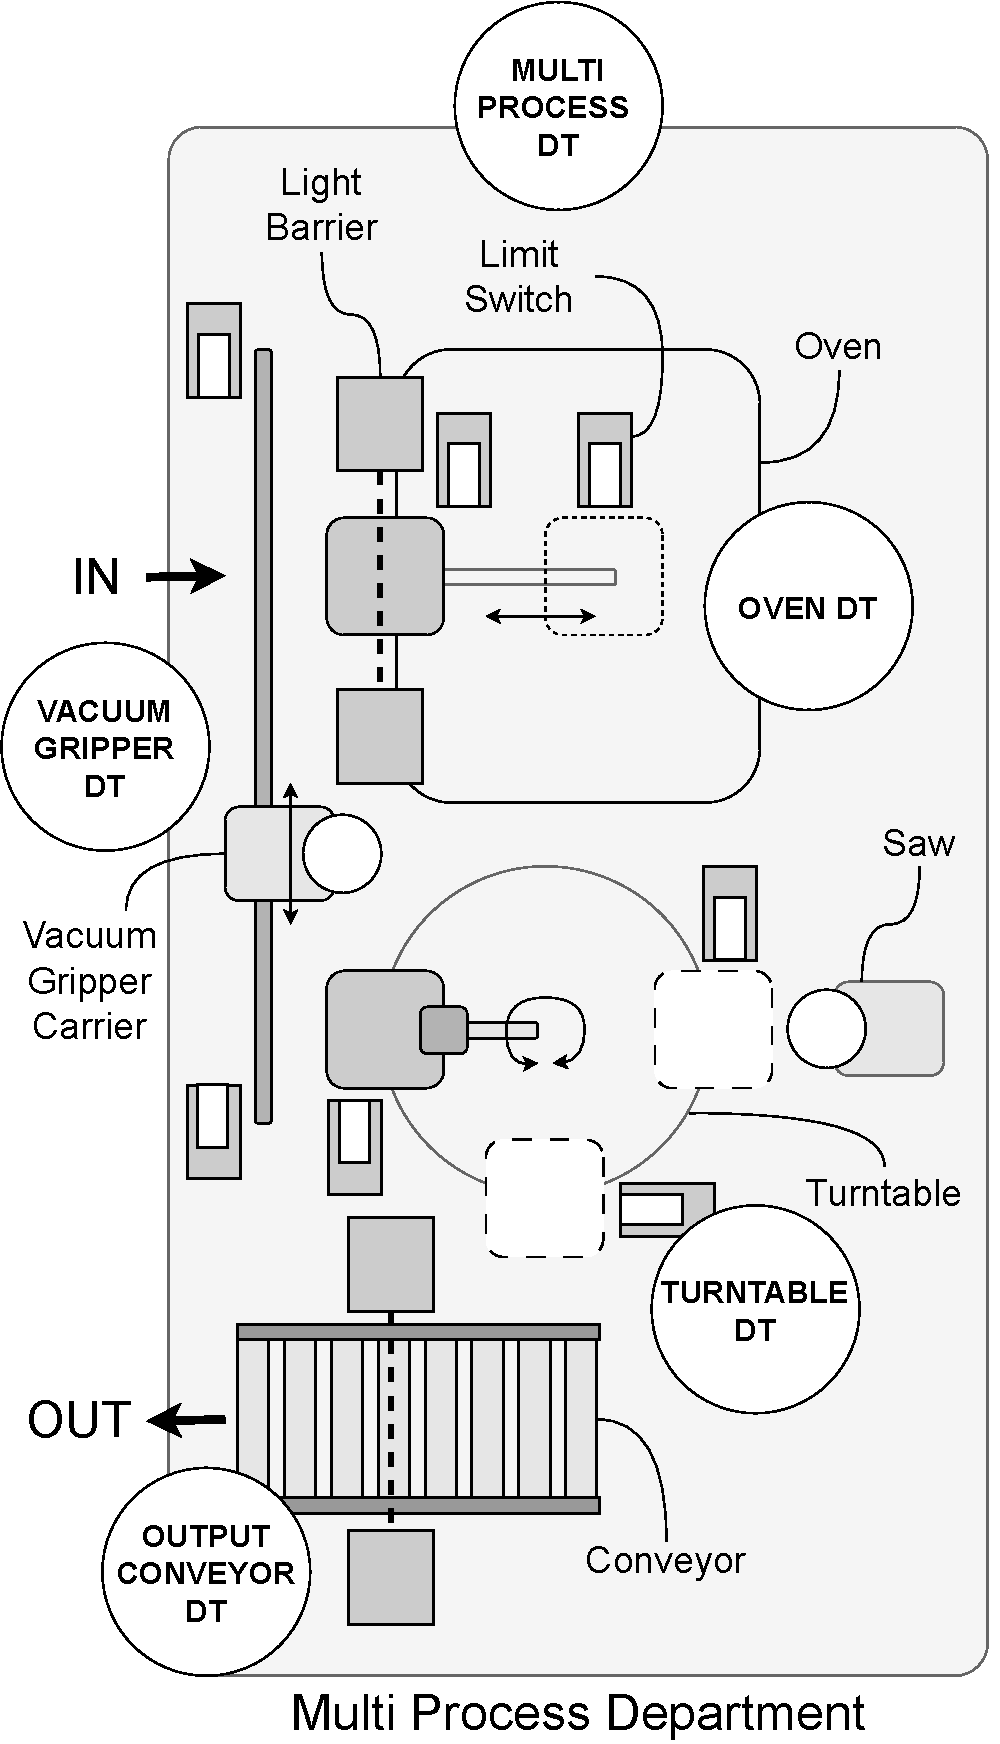
\includegraphics[width=0.9\columnwidth]{figures/dt-lifecycle/multiprocess-station-shcematic-overview.pdf}
    \caption{Multi-process Station schematic overview.}
    \label{fig:multiprocess-station-schematic-overview}
\end{figure}

\begin{figure}
    \setlength{\belowcaptionskip}{-13pt}
    \centering
    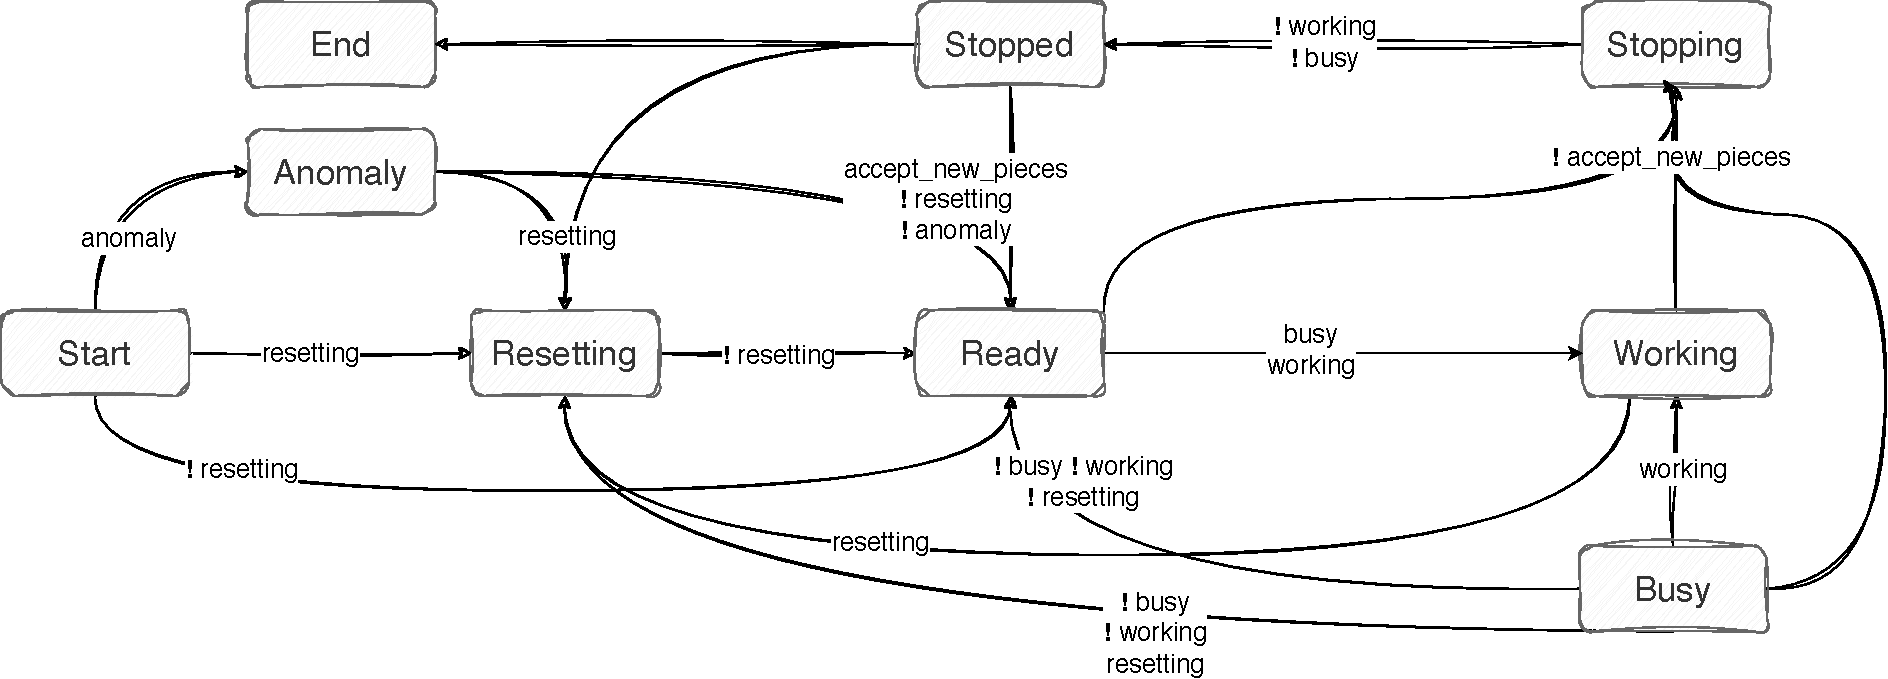
\includegraphics[width=\textwidth]{figures/dt-lifecycle/graph_machine_logic.pdf}
    \caption{Machine DT Lifecycle with a focus on the different phases in the Synchronization state.}
    \label{fig:graph-machine-logic}
\end{figure}

\subsection{DT Design \& Development}

The design, development, and deployment of Digital Twins (DTs) for the target use case are motivated by the need for precise monitoring, control, and optimization of physical machinery and stations. By creating digital replicas of the physical systems, we aim to enhance operational efficiency, reduce downtime, and enable predictive maintenance through detailed real-time data analysis and simulation capabilities.

To achieve these objectives, multiple DTs have been designed, developed, and deployed to represent the associated Physical Twins (PTs). Specifically, each station was divided into several processing machines, with a DT created for each one. Subsequently, a \textit{composed} DT was developed for each station to aggregate data from the individual machine DTs, enabling a complete digital representation of the station. This allows for the monitoring and management of the combined operations of multiple physical assets working together through the production process. For example, Figure \ref{fig:multiprocess-station-schematic-overview} illustrates the schematic representation of the Multiprocess Station along with the DTs it comprises.

The DTs were implemented using the White Label Digital Twin (WLDT)\footnote{WLDT Library: \url{https://wldt.github.io/}} library~\cite{wldt_picone_2021}. WLDT is a Java implementation of an event-driven DT framework that supports data ingestion through IoT interfaces and message queues. We extended the library to support the proposed lifecycle management approach by implementing both the Physical Twin Lifecycle ($LP_{PT}$) and the Digital Twin Lifecycle ($LP_{DT}$). Each DT features various adapters for external communication, including both physical and digital interfaces. For physical interface management, the DTs controlling individual machines use an OPC-UA\footnote{OPC-UA-Foundation: \url{https://opcfoundation.org/}} adapter, which enables interaction with Siemens S7-1200 PLCs\footnote{Siemens-S7-1200-PLC:\url{https://www.siemens.com/global/en/products/}}. Additionally, each DT includes MQTT\cite{mqtt} Digital and HTTP Digital adapters to expose both its current state and the lifecycle's phases it represents through different protocols and interaction patterns (Pub/Sub and RESTful).

Each machine DT handles the synchronization between the $LP_{PT}$ and the corresponding $LP_{DT}$. Furthermore, an anomaly detection algorithm runs within each DT, enabling it to identify and report issues that the PLC alone might not detect, thus dynamically computing the $LP_{PT}$ when necessary (e.g., when a piece does not reach a reference photocell on the machinery within a predetermined time and an anomaly is consequently detected).

The DTs also calculate the \textit{Overall Equipment Effectiveness} (OEE)\footnote{OEE: \url{https://www.oee.com/}}, a key efficiency metric in the industrial domain that measures the productivity of manufacturing equipment by combining its availability, performance, and quality rates. We compute OEE in our DTs to provide a comprehensive measure of equipment effectiveness, which is critical for identifying areas of improvement and optimizing production processes. This data is exposed for external monitoring.

The composite DT uses an MQTT adapter as its physical interface to collect data and lifecycle phases from the individual machine DTs. It incorporates coordination logic that adjusts machine behavior based on their current phases, ensuring seamless station management. Additionally, the composite DT has its own MQTT Digital and HTTP Digital adapters to expose the station’s overall state externally. The described DT structure is illustrated in Figure \ref{fig:multiprocess-station-dt-structure}.

The DTs of the machines operate based on data produced by their physical counterparts. This data originates from readings of all sensors present on the machinery, along with the states of its actuators. These data are mapped to the DT state, ensuring that at any given moment, the DT reflects the state of the physical object. Leveraging these temporal data, it was possible to model the lifecycle of the physical object within the DT lifecycle.

When the DT lifecycle reaches the Synchronized state, it accurately mirrors the corresponding phase of the physical machinery's operation. The modeled lifecycle, as shown in Figure \ref{fig:graph-machine-logic}, outlines the generic phases defined for each machine. These phases not only reflect the actual operation of the machinery but are also inspired by the reference structure for industrial machine phases defined by ISA-95\footnote{ISA-95:https://www.isa.org/standards-and-publications/isa-standards/isa-standards-committees/isa95}. This alignment ensures that our DTs adhere to recognized industry standards, enhancing their applicability and effectiveness in real-world industrial settings.

To accurately define the phases of the physical machinery, it was essential to specify the transition conditions between these phases by leveraging the raw data and telemetry received from sensors and actuators via OPC-UA from the PLC. The DT processes this data to compute and maintain the synchronized lifecycle, ensuring a precise and real-time reflection of the physical object's operational state. This approach enables the DT to seamlessly transition between phases based on the actual conditions and performance of the machinery, providing an accurate digital representation.

\begin{figure}[ht]
    \setlength{\belowcaptionskip}{-13pt}
    \centering
    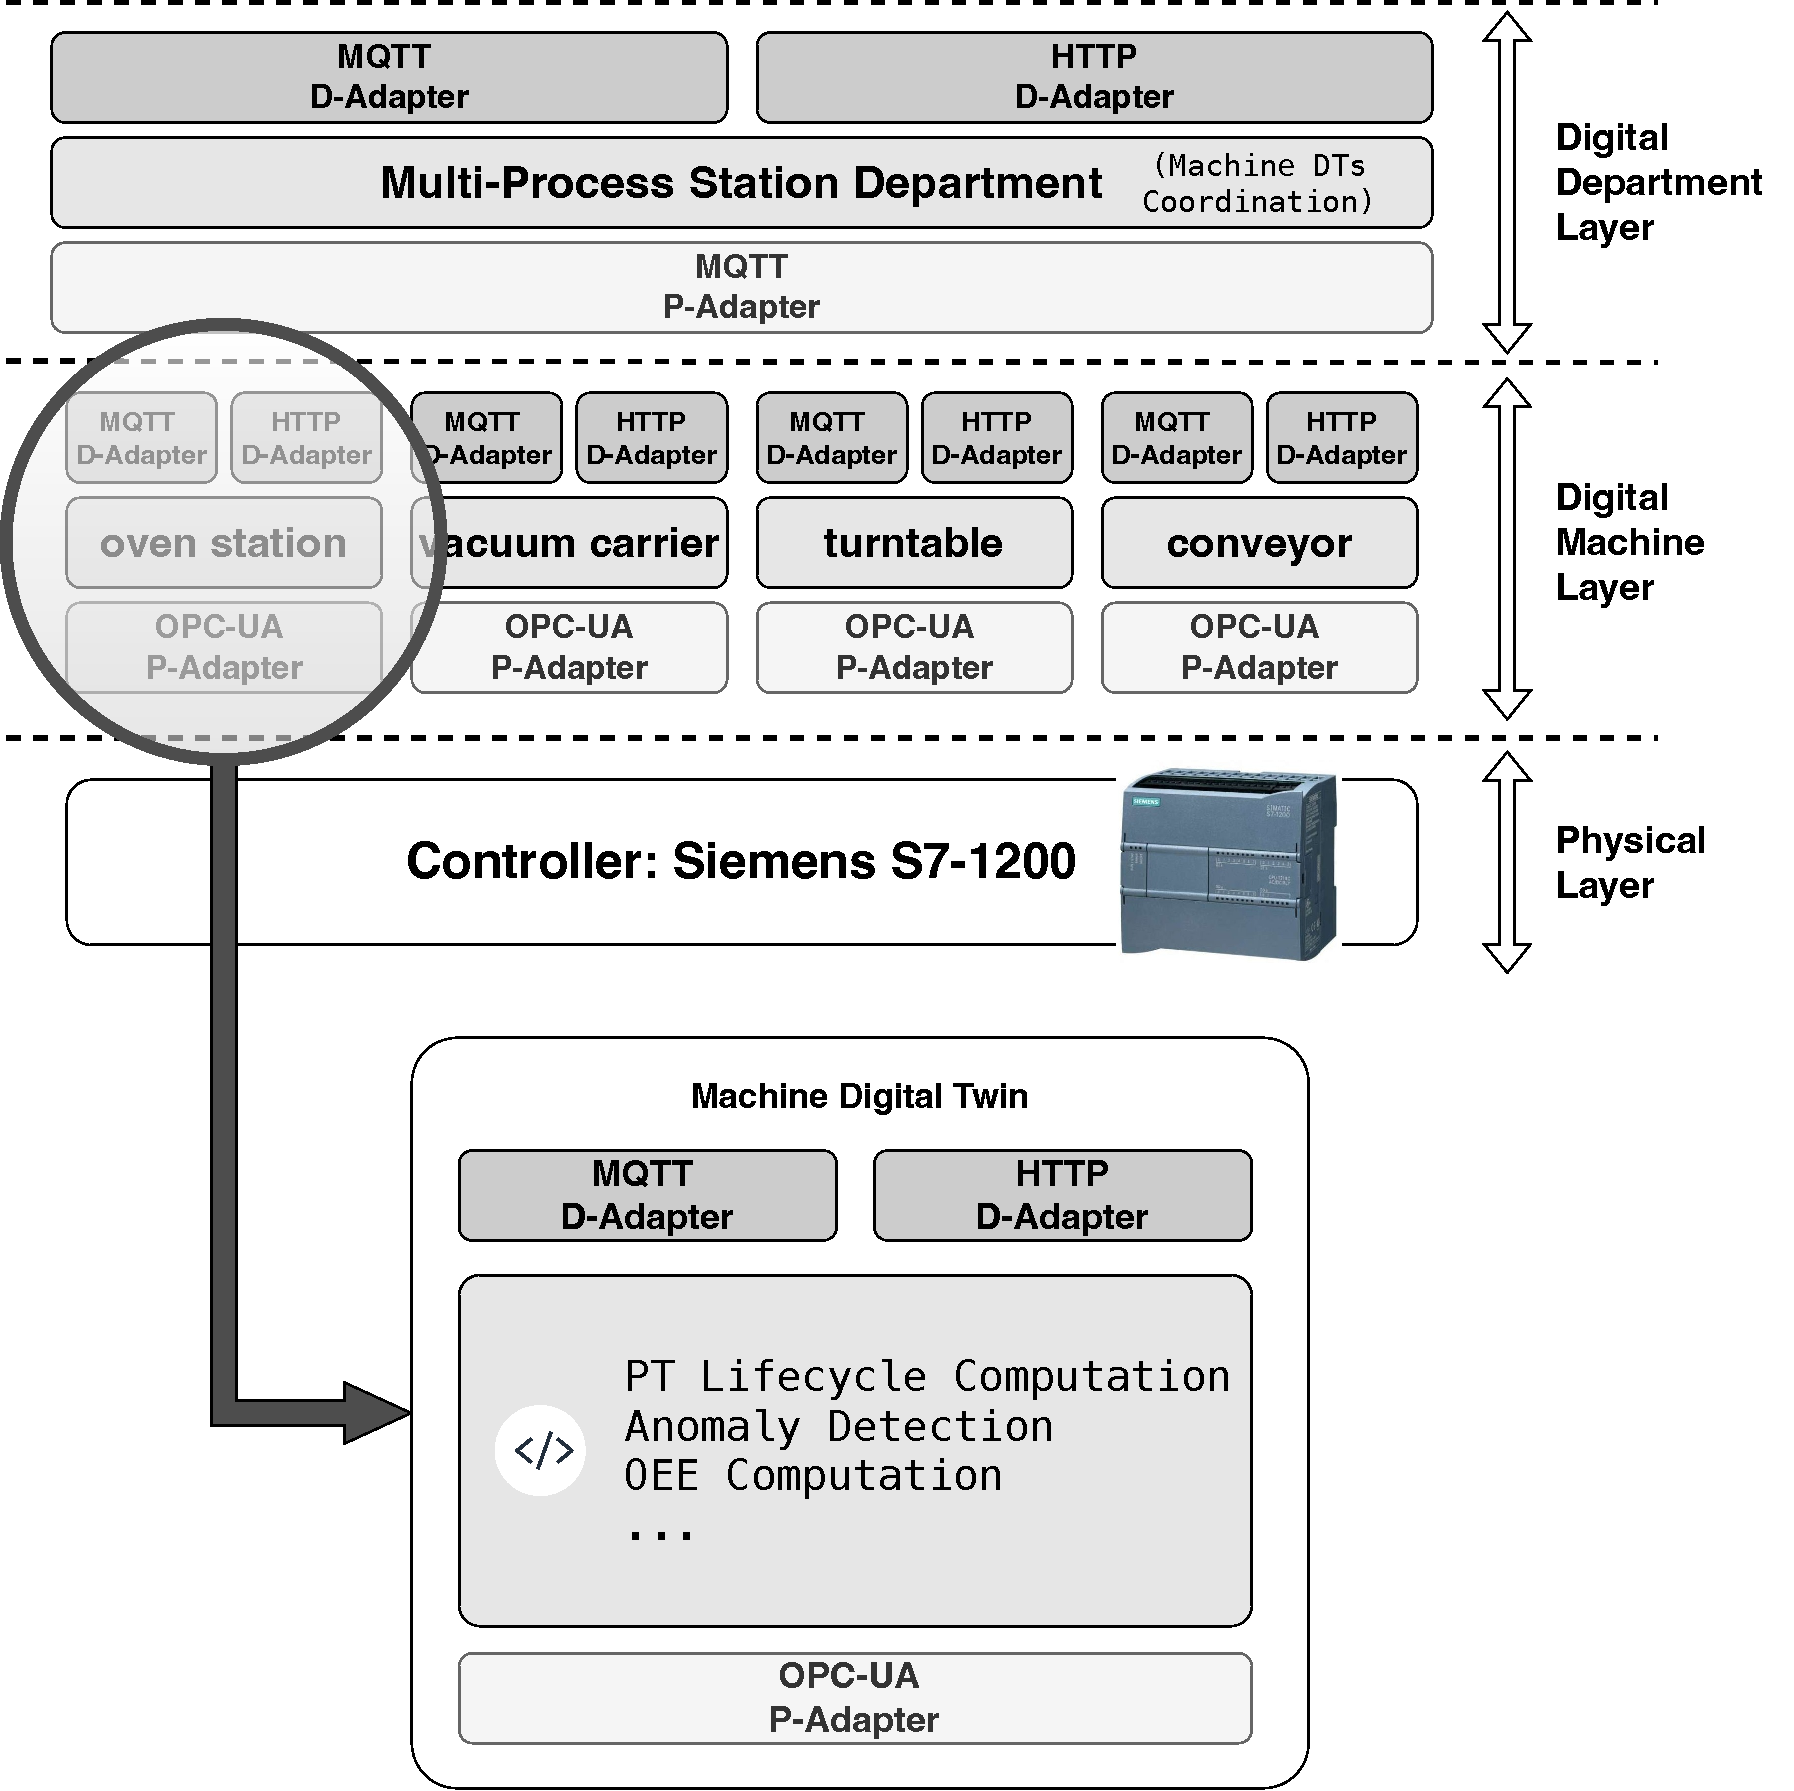
\includegraphics[width=\columnwidth]{figures/dt-lifecycle/mps_dt_structure_2.pdf}
    \caption{Multi-process Station Digital Twin overview.}
    \label{fig:multiprocess-station-dt-structure}
\end{figure}

\subsection{Lifecycle Awareness \& Coordination}

In an industrial setting, the digital representation of a station is often a hierarchical composition of individual machines, each represented by its own DT. This structure enables intelligent coordination not only between machines within the same station but also across different stations. For example, coordination between the \textit{Multiprocess Station} and the previously mentioned \textit{Indexed Line} becomes more manageable compared to a direct access to low level raw data of the different physical machines. Incorporating the PT lifecycle into the DT lifecycle simplifies coordination by establishing consistent lifecycle phases across machines.
Without this approach, coordination among multiple DTs required using low-level physical information and telemetry, making the process more complex and less intuitive. Now, as illustrated by Algorithm \ref{code:soft-stop-logic}, high-level control logic can be implemented directly leveraging information encapsulated by $LP_{DT}$ mapping in real-time the phase and the associated transitions of the associated physical counterparts $LP_{PT}$. Specifically, the algorithm outlines the steps the composite DT can take to halt production on the multiprocess station. By leveraging this additional layer of abstraction, the composite DT no longer relies on raw sensor data for control operations, enabling a more declarative and effective coordination process, and distributing responsibilities across different DTs.

The composite DT leverages the PT lifecycle phases of individual machines to define the overall lifecycle of the entire multiprocess station. This provides a comprehensive overview of each station's operational behavior, enabling more effective and intuitive system management.

\note{FIX ALGORITHM}
% \begin{algorithm}
% \caption{Multiple DTs Stopping Procedure}
% \begin{algorithmic}
% \State \texttt{invoke(OvenDT, STOP)}
% \While{ \texttt{OvenDT.phase} \textbf{is not} \texttt{STOPPED} }
%     \State \texttt{wait(OvenDT.phase} \textbf{is not} \texttt{WORKING)}
% \EndWhile
% %\vspace{1em}
% %\State \textbf{publish} event ``change-vacuum-gripper-cycle" with value \texttt{false}
% \State \texttt{invoke(GripperDT, STOP)}
% \While{ \texttt{GripperDT.phase} \textbf{is not} \texttt{STOPPED}}
%     %\State \textbf{log} waiting for end of vacuum-gripper \texttt{WORKING} state
%     \State \texttt{wait(GripperDT.phase} \textbf{is not} \texttt{WORKING)}
% \EndWhile
% %\vspace{1em}
% %\State \textbf{publish} event ``change-turntable-cycle" with value \texttt{false}
% \State \texttt{invoke(TurntableDT, STOP)}
% \While{ \texttt{TurntableDT.phase} \textbf{is not} \texttt{STOPPED} }
%     %\State \textbf{log} waiting for end of turntable \texttt{WORKING} state
%     \State \texttt{wait(TurntableDT.phase} \textbf{is not} \texttt{WORKING)}
% \EndWhile
% %\vspace{1em}
% \State \texttt{invoke(OutputConveyorDT, STOP)}
% \end{algorithmic}
% \label{code:soft-stop-logic}
% \end{algorithm}



\subsection{Industrial Digital Twins with WLDT}
\label{sec:industrial-dt-wldt}

The proposed DT architectural approach has been initially applied and validated in a realistic industrial environment: a microfactory which serves as an experimental platform for DTs and industrial ecosystems. The industrial environment has been strategically chosen since it represents one of the most challenging application scenarios for DTs, characterized by stringent requirements in terms of integration with heterogeneous systems, and the management of fragmented data through multiple stakeholders. 

However, it is crucial to emphasize that the proposed approach is inherently flexible and designed to be applicable in a wide spectrum of other  contexts. While the initial validation focused on the industrial domain we foster the application of our framework in other domains and use cases, such as Smart Cities \cite{10.1145/3570361.3614070} and Health \cite{9325551} where the concepts of DTs can bring significant value. The modularity and scalability of our solution facilitate its adoption in various types of applications, and future work may explore in detail its effectiveness in these additional contexts.

Specifically, the validation in the industrial domain was carried out using the \emph{Fischertechnik Training Factory Industry 4.0}\footnote{Fischertechnik Industry \& Universities: \url{https://www.fischertechnik.de/en/products/industry-and-universities}} Indexed-Line Station, featuring the \emph{Multiprocess Station with Oven} module.
This microfactory setup provides a controlled yet dynamic environment for testing and refining DT technologies in a realistic industrial context.

%%%
\begin{figure*}
    \setlength{\belowcaptionskip}{-13pt}
    \centering
    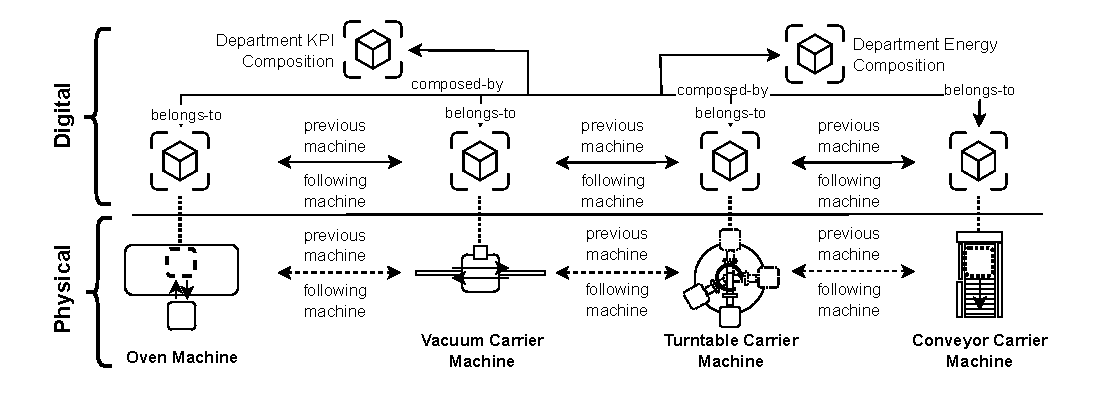
\includegraphics[width=0.92\textwidth]{figures/engineering-wldt/Fischer-relationships.pdf}
    \caption{DTs relationships with both those existing in the physical space as well those belonging to the digital composition.}
    \label{fig:dt-assets-relationships-overview}
\end{figure*}
%%%

As shown in Figure~\ref{fig:discher-dt-first-level}, the module consists of five machines arranged in a flow shop layout: three material handling units (vacuum gripper carrier, turntable, and conveyor) and two transformation stations (oven and saw station).
Each machine is equipped with sensors (light barriers and limit switches) and actuators (with two or three operational states), all managed by a 24V industry-grade digital board.
A Raspberry Pi-based soft-PLC, connected to a 24V Digital I/O expansion board, controls the system and coordinates machine operations via sensors and actuators. Real-time process data is published to an MQTT broker DTs can subscribe to to receive data.

The digitalization goal is to monitor the state, track production performance and power consumption, and regulate the production speed of each machine through a DT.
Additionally, to compute the overall production performance and manage external action requests, and to track the overall power consumption, two department-level DTs are created, matching the two different modeling goals.
Each machine-level DT processes incoming data on properties and events to generate insights such as production and energy KPIs, while also managing action requests to regulate their individual speed.
Relationships between DTs are crucial, as they represent connections between physical assets, which can be used by external applications and other DTs, facilitating \emph{compositions} to form higher-level DTs.

% The digitalization of the department begins with the machine layer, using DT compositions to create higher-level DTs. To capture different aspects of the department (e.g., overall production performance and energy consumption), machine-level DTs can be integrated into two distinct department-level compositions, each specializing in one of the targeted aspects.

% This specialization is achieved by selecting specific information in the DT configuration and using the department DT model to manipulate, augment, and output relevant information. Department-level DTs, structured similarly to machine-level DTs, handle action requests through their internal models, just like the lower-level DTs. Relationships maintain their importance, representing actual connections between the department DT (whether specialized in performance or energy tracking) and other DTs within the system.

%%%

\subsection{Machines Digital Twins}
\label{subsec:dt-machine-level} 

The digitalization process creates five machine-level DTs, one for each machine in the factory (Figure~\ref{fig:discher-dt-first-level}). These DTs each interact via an MQTT broker through the PI, are equipped with an internal model implemented by the Shadowing Function, and have a Digital Interface to share data.
The DT ecosystem digitalizes the physical system without replacing the PLC logic, allowing for the independent operation of the PLC if the DT ecosystem fails.
DTs are deployed on edge nodes for monitoring and control without disrupting core operations.

Each DT connects to the broker through MQTT Physical Adapters, which manage subscriptions to relevant topics and publish the description of PTs. The internal model of each DT calculates metrics like OEE (based on production rate, uptime, downtime, and quality) and tracks power consumption. Relationships between machines and DTs (e.g., \emph{previous}, \emph{following-machines}, \emph{is-part-of}) are defined at startup and remain static during the experiment.
Machine DT states are exposed via MQTT and HTTP Digital Adapters, enabling flexible interaction patterns and action requests through HTTP.

%%%
\begin{figure*}
    \setlength{\belowcaptionskip}{-13pt}
    \centering
    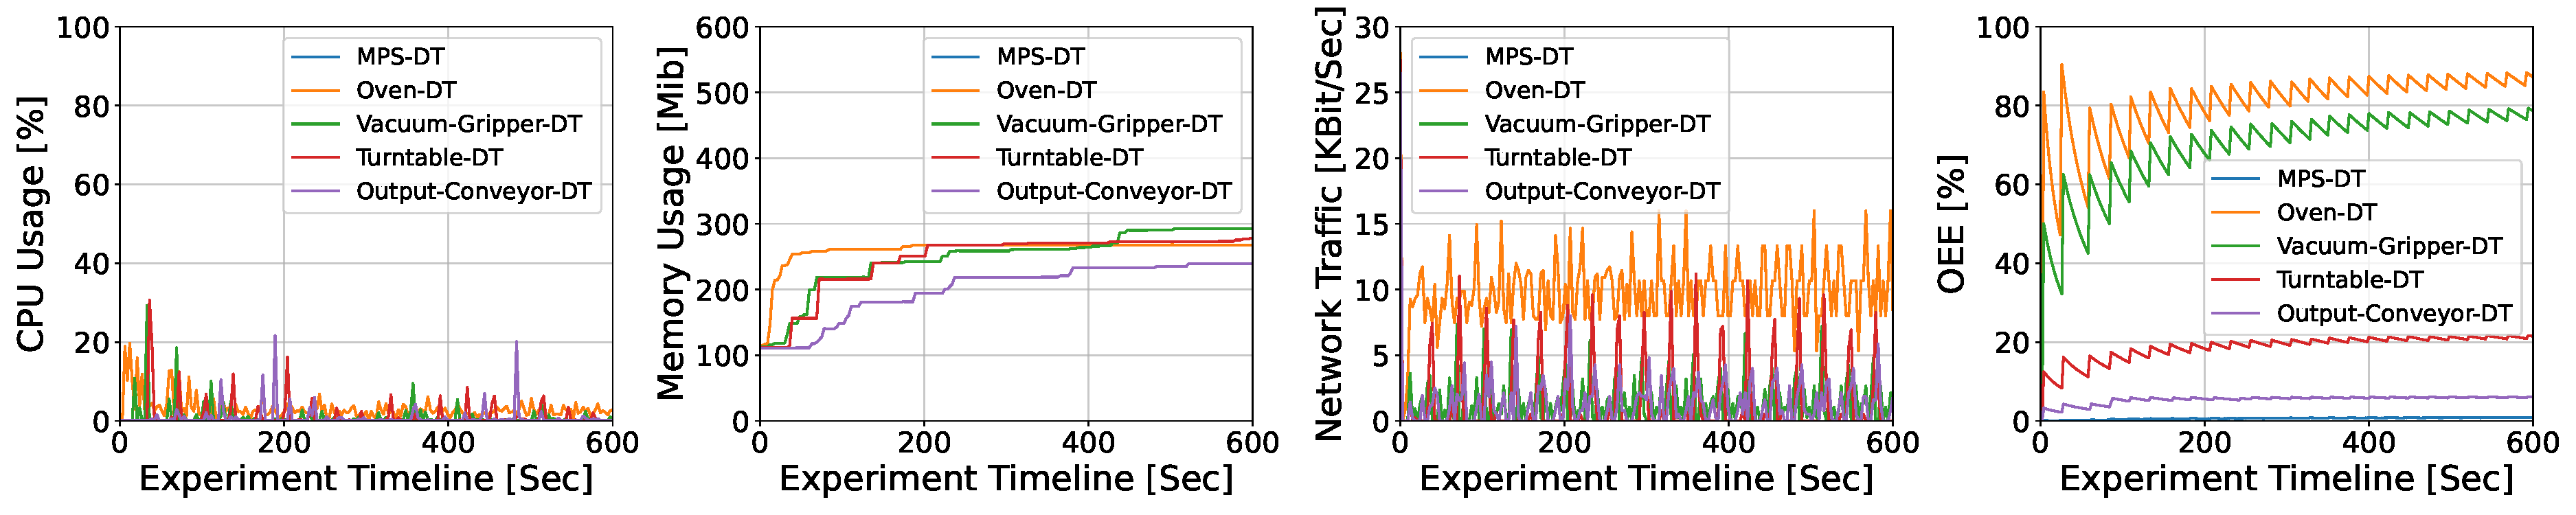
\includegraphics[width=\textwidth]{figures/engineering-wldt/experimental_results.pdf}
    \caption{Experimental Results: CPU usage percentage [\%], Memory usage [Mib], Network usage [KBit/sec] and OEE [\%]}
    \label{fig:exp-results}
\end{figure*}
%%%

%%%

\subsection{Department Digital Twins}
\label{subsec:dt-department-level}

The identified department DTs model and monitor KPIs and energy metrics based on the machine DTs structure. The Department KPI DT focuses on tracking performance, including weighted OEE and throughput. Weighted OEE is calculated using OEEs received from each machine DT~\cite{OEE-manufacturing-cell-Gamberini-2017}.
Throughput, defined as the number of processed pieces per time unit in production systems, is tracked by monitoring entry and exit events of pieces processed by machines within the department, facilitated by relationships in the DT ecosystem.

The Department-KPI DT tracks piece processing start and completion, calculates throughput, and monitors total pieces processed.
Relationships between lower and upper-level DTs are shown in Figure~\ref{fig:dt-assets-relationships-overview}.
The Department DT accepts action requests via its HTTP digital adapter, adjusting production rates through its Shadowing Function, which cascades actions to underlying DTs and physical assets.
The Department-Energy DT monitors energy consumption, aggregating data from machine-level DTs, and processes it through an internal model to derive target metrics.
It also uses an HTTP digital adapter for external interaction.
Department-level DTs use MQTT-based physical adapters to ensure consistent communication and enable external applications to coordinate actions across the underlying DT instances.

% The Department-KPI DT can track the start and completion of piece processing, calculate throughput based on time per piece, and total pieces processed. Relationships between lower-level and upper-level DTs are illustrated in Figure~\ref{fig:dt-assets-relationships-overview}. The Department DT accepts action requests via its HTTP digital adapter, supporting operations to adjust production rates. Speed changes are processed through a simple algorithm in the Department DT's Shadowing Function, cascading actions to underlying DTs and associated physical assets. The Department Energy DT monitors overall energy consumption, aggregating data from machine-level DTs regardless of whether it's specific energy consumption or disaggregated voltage and current data. Its internal model handles this heterogeneity to derive target metrics. The Department Energy DT also utilizes an HTTP digital adapter for external interaction, providing access to its internal state information. Department DTs utilize MQTT physical adapters within their physical interface, ensuring consistent implementation of composed DTs. They enable external applications to interact with the department through HTTP digital adapters, managing actions across underlying DTs based on the department's internal model and behavior.


%%%
% \begin{figure*}
%     \centering
%     \setlength{\belowcaptionskip}{-13pt}
%     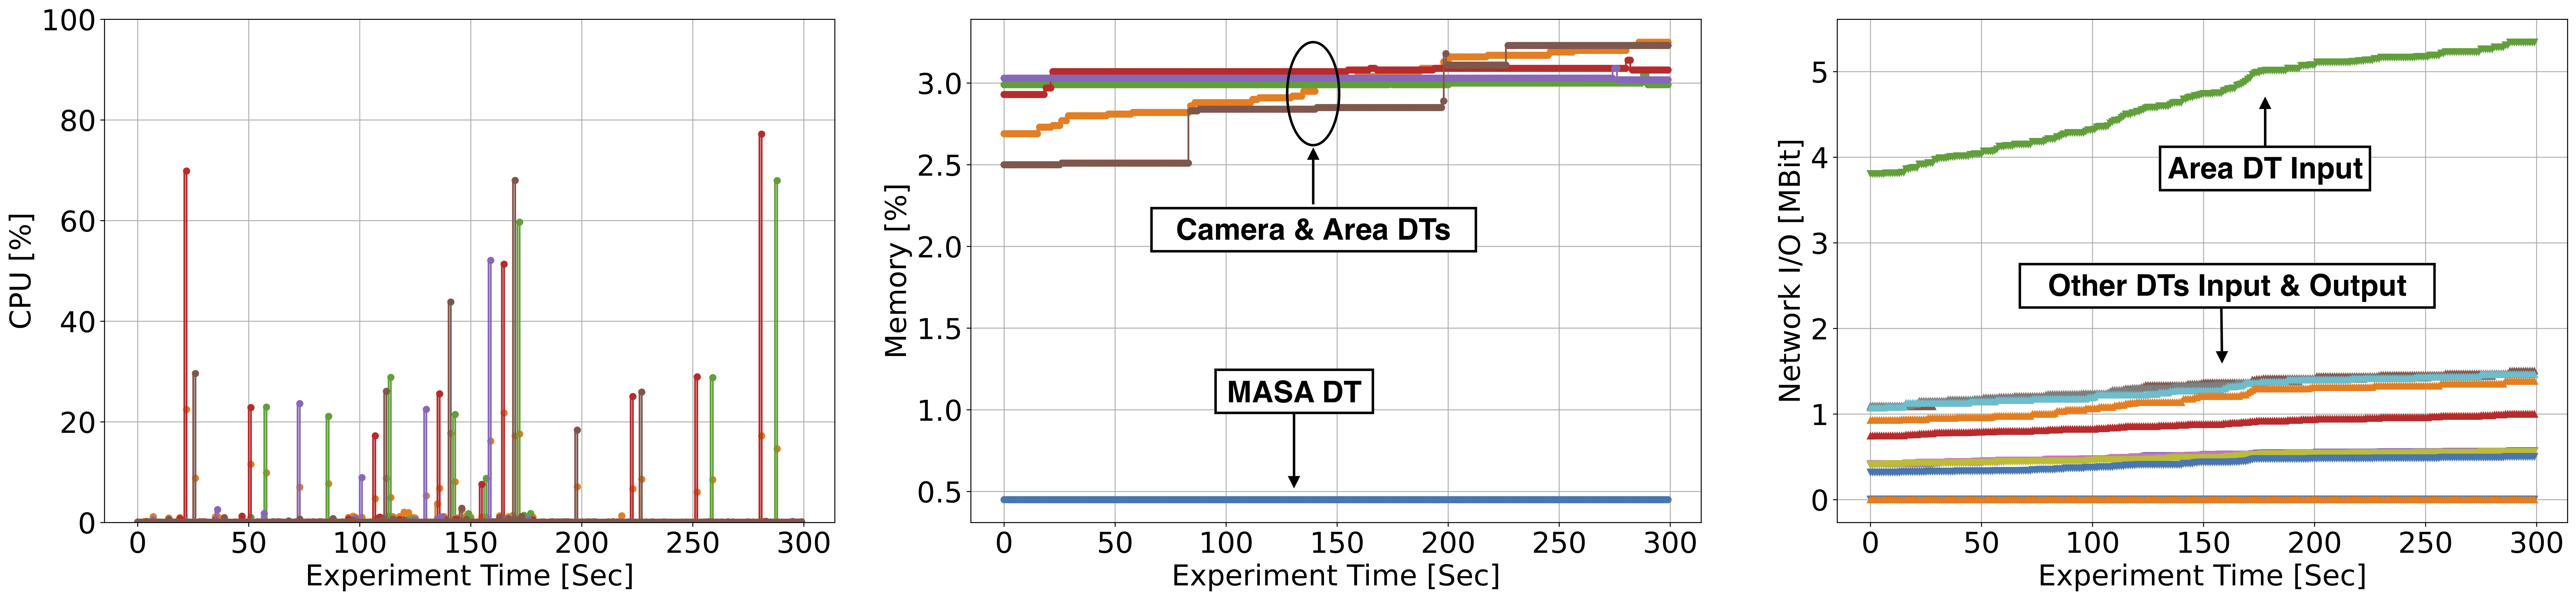
\includegraphics[width=\textwidth]{images/masa_dt_result.png}
%     \caption{Experimental evaluation of the MASA DT deployment with CPU\%, Memory usage\% and the cumulative Network I/O.}
%     \label{fig:masa_dt_results}
% \end{figure*}
%%%

\subsection{Experimental Evaluation}
\label{ssec:masa_exp_evaluation}

To validate the WLDT framework, we implemented the DTs for the Multiprocess Station with Oven, containerized using Docker, and deployed on an Edge node with an Intel i7 2.4GHz processor and 32 GB of RAM. We monitored three key metrics for each DT: CPU usage (percentage, with each container using one core), memory consumption (in MiB), and network traffic (cumulative inbound and outbound in Kbit/sec).
Additionally, we calculated the OEE computed by each DT to assess the performance of both individual machines and the station. Figure \ref{fig:exp-results} shows the results of this experiment. The total duration was 10 minutes (600 seconds), as shown on the x-axis of each chart. The graphs illustrate CPU usage, memory usage, network traffic, and the computed OEE (from left to right). Analyzing CPU usage, we observe that there were no significant spikes during the production cycle. Even during the most computationally demanding moments, CPU utilization remained around 30\%, indicating a stable and efficient execution.
The memory usage chart shows a similarly stable pattern, with DT instances settling around an average usage of 300 MiB, demonstrating consistent memory behavior over time.
As for network traffic, values remained low—typically around a few tens of Kbit/sec.
Noticeable traffic peaks correspond to active processing phases, where machines and their respective DTs exchange larger volumes of data.
Finally, the OEE graph highlights the performance of industrial machines computed by each DT. The Oven, which is the first machine in the station and requires the longest processing time, shows the highest OEE, as it remains under constant workload.
Conversely, the output conveyor exhibits a lower OEE, as it receives fewer parts to process due to the upstream bottleneck created by the Oven. This experimental phase aimed to demonstrate the effectiveness of WLDT-based DTs in an industrial setting.
The collected metrics confirm that DT instances can operate efficiently on standard commercial Edge nodes, handling CPU, memory, and network constraints while also supporting domain-specific computations such as OEE. These results validate the potential of the WLDT framework for practical DT development and deployment in real-world industrial scenarios.